\documentclass[12pt,a4paper,titlepage,listof=totoc,bibliography=totoc,chapteratlists=0pt]{scrreprt}

\begin{filecontents*}{\jobname.xmpdata}
	\Keywords{VR, IOT, TODO}
	\Title{Machine Learning In Microsoft Azure - Einseitige Aufarbeitung}
	\Author{Emina Sljivic}
\end{filecontents*}

\setcounter{tocdepth}{1}

\usepackage[utf8]{inputenc}
\usepackage[T1]{fontenc}
\usepackage{amsmath}
\usepackage{amsfonts}
\usepackage{amssymb}
\usepackage[table]{xcolor}
\usepackage{graphicx}
\usepackage[left=3.50cm, right=2.00cm, top=2.00cm, bottom=2.00cm,foot=1cm]{geometry}
\usepackage[splitrule,hang,flushmargin,multiple,bottom]{footmisc}
\usepackage{lmodern, textcomp}
\usepackage{lmodern}
\usepackage{pdfpages}
\usepackage{multicol}
\usepackage{subfig}
\usepackage{float}
\usepackage{array,tabularx,booktabs}
\usepackage{ragged2e}
\usepackage{lipsum}
\usepackage{wrapfig}
\usepackage{tabularx}

\newcolumntype{M}[1]{>{\centering\arraybackslash}m{#1}}

\usepackage{enumitem}
\newlist{compactitem}{itemize}{3}
\setlist[compactitem,1]{label=\textbullet, nosep,leftmargin=1.5em,labelwidth=*,align=left}
\setlist[compactitem,2]{label=--, nosep,leftmargin=1.5em,labelwidth=*,align=left}
\setlist[compactitem,3]{label=\textopenbullet, nosep,leftmargin=1.5em,labelwidth=*,align=left}
\newlist{compactenum}{enumerate}{3}
\setlist[compactenum,1]{label=\arabic*., nosep,leftmargin=1.5em,labelwidth=*,align=left}
\setlist[compactenum,2]{label=\alph*., nosep,leftmargin=1.5em,labelwidth=*,align=left}
\setlist[compactenum,3]{label=\roman*., nosep,leftmargin=1.5em,labelwidth=*,align=left}
\newlist{compactdesc}{description}{3}
\setlist[compactdesc]{leftmargin=1.5em,labelwidth=*,align=left}

\usepackage{microtype}

\usepackage[parfill]{parskip}

\definecolor{bluekeywords}{rgb}{0.13,0.13,1}
\definecolor{greencomments}{rgb}{0,0.5,0}
\definecolor{redstrings}{rgb}{0.9,0,0}
\definecolor{lightgray}{gray}{0.9}
\definecolor{lightblue}{rgb}{0.93,0.95,1.0}

\usepackage{listings}

\makeatletter
\lstdefinestyle{lststyle}{
	basicstyle=%
	\ttfamily
	\lst@ifdisplaystyle\scriptsize\fi
}
\makeatother

\renewcommand{\lstlistlistingname}{List of Listings}
% TODO: define other languages as needed
\lstset{language=Python,
	numbers=left,
	numberstyle=\tiny,
	showspaces=false,
	showtabs=false,
	breaklines=true,
	lineskip=-1pt,
	tabsize=2,
	showstringspaces=false,
	breakatwhitespace=true,
	escapeinside={(*@}{@*)},
	commentstyle=\color{greencomments},
	keywordstyle=\color{bluekeywords}\bfseries,
	stringstyle=\color{redstrings},
	style=lststyle,
	xleftmargin=17pt,
	framexleftmargin=17pt,
	framexrightmargin=5pt,
	framexbottommargin=4pt
}
\lstset{
	morekeywords={base,var,in,out,dynamic,from,where,select,orderby,function,\$,group,by,into,yield,async,await,@,None,self,as,elif,with}
}
\lstdefinelanguage{TypeScript}{
	keywords={typeof, new, true, false, catch, function, return, null, switch, var, if, in, while, do, else, case, break, void, number, string, boolean, module, \$, export, for, this},
	keywordstyle=\color{blue}\bfseries,
	ndkeywords={class, export, boolean, throw, implements, import, this},
	ndkeywordstyle=\color{darkgray}\bfseries,
	identifierstyle=\color{black},
	sensitive=false,
	comment=[l]{//},
	morecomment=[s]{/*}{*/},
	commentstyle=\color{purple}\ttfamily,
	stringstyle=\color{red}\ttfamily,
	morestring=[b]',
	morestring=[b]"
}
\usepackage{caption}
\DeclareCaptionFont{white}{\color{white}}
\DeclareCaptionFormat{listing}{\colorbox[cmyk]{0.43, 0.35, 0.35,0.01}{\parbox{\textwidth}{\hspace{10pt}#1#2#3}}}
\captionsetup[lstlisting]{format=listing,labelfont=white,textfont=white}
\captionsetup[table]{justification=centering, singlelinecheck=false}

\usepackage{setspace}
\newcommand{\MSonehalfspacing}{%
	\setstretch{1.44}%  default
	\ifcase \@ptsize \relax % 10pt
		\setstretch {1.448}%
	\or % 11pt
		\setstretch {1.399}%
	\or % 12pt
		\setstretch {1.433}%
	\fi
}

\newcommand{\setauthor}[1]{\ohead[]{#1}}

\usepackage[automark]{scrlayer-scrpage}
\pagestyle{scrheadings}
\automark{chapter}
\renewcommand\sectionmark[1]{\markright{\MakeMarkcase {\thesection\hskip .5em\relax#1}}}
\rohead{\ifnum\expandafter\pdfstrcmp\botmark=0 \rightmark\else\leftmark{} --- \rightmark\fi}
\ihead[]{\headmark}
\chead[]{}
\ohead{}
\cfoot[]{}
\ofoot[\pagemark]{\pagemark}
\setheadsepline{.1pt}

\usepackage[hyphens]{url}

\usepackage[a-1b]{pdfx}

\usepackage{hyperref}
\hypersetup{pdfa}

\usepackage[nonumberlist,toc,nopostdot]{glossaries}

\usepackage{chngcntr}
\counterwithout{footnote}{chapter}
\counterwithout{figure}{chapter}
\counterwithout{table}{chapter}
\AtBeginDocument{
	\counterwithout{lstlisting}{chapter}
	\urlstyle{sf}
}
\newcounter{RPages}

\makeatletter
\def\bstctlcite{\@ifnextchar[{\@bstctlcite}{\@bstctlcite[@auxout]}}
\def\@bstctlcite[#1]#2{\@bsphack
	\@for\@citeb:=#2\do{%
		\edef\@citeb{\expandafter\@firstofone\@citeb}%
		\if@filesw\immediate\write\csname #1\endcsname{\string\citation{\@citeb}}\fi}%
	\@esphack}
\makeatother

\clubpenalty=10000
\widowpenalty=10000
\displaywidowpenalty=10000
\interfootnotelinepenalty=10000

\title{Machine Learning In Microsoft Azure - Einseitige Aufarbeitung}
\author{Sljivic Emina}

\makeindex
\makeglossaries

\usepackage[OT2, T1]{fontenc}
\usepackage[russian, ngerman]{babel}
\begin{document}
\bstctlcite{IEEEexample:BSTcontrol}
\newcommand{\reminder}[1]
{ \textcolor{red}{<[{\bf\marginpar{\mbox{$<==$}} #1 }]>} }
\newcommand{\icode}[1]{\lstinline$#1$}
%\urlstyle{same}
%\setstretch{1.5}
\setstretch {1.433}
\renewcommand{\arraystretch}{1.5}

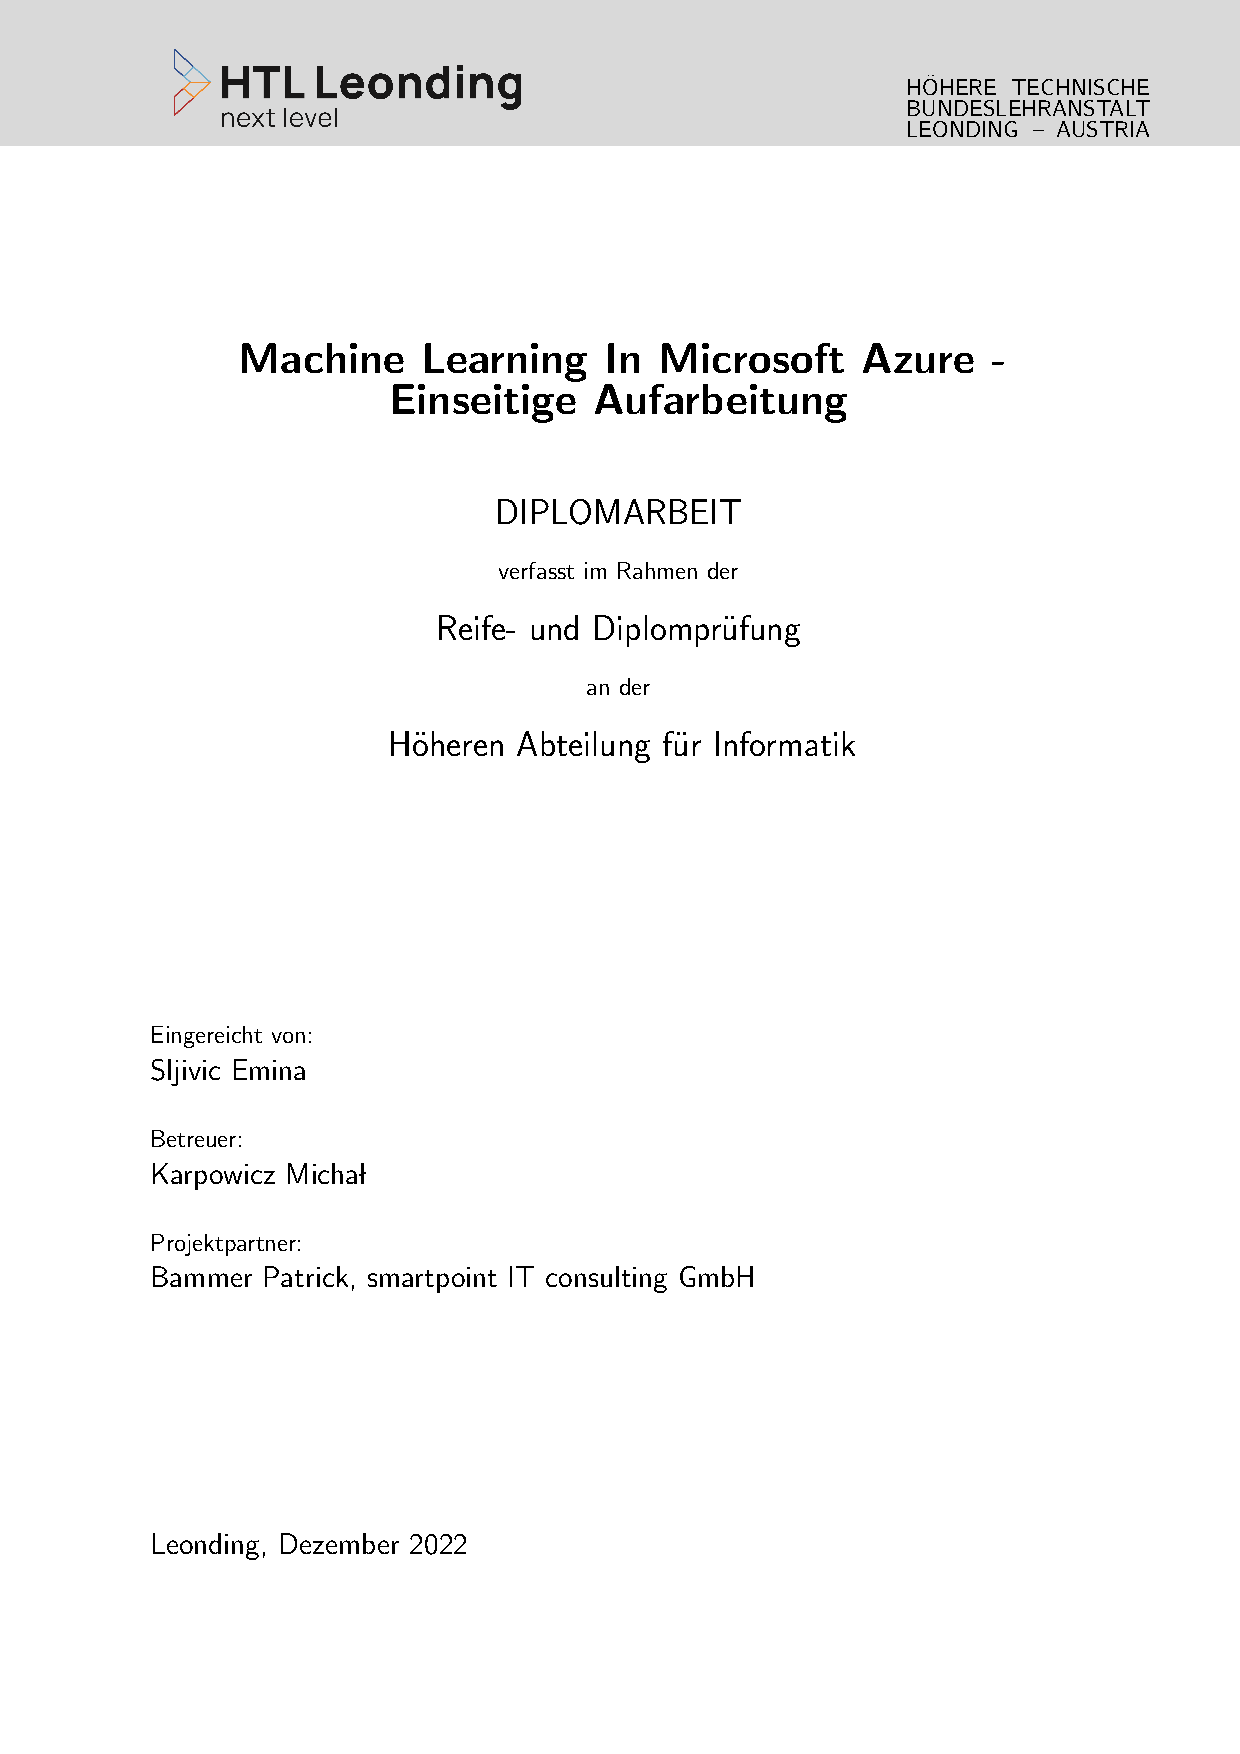
\includepdf{./titlepage/coversheet}
\pagenumbering{Roman}
\newpage
\thispagestyle{empty}
\vspace{3cm}
~ \\ \\
Ich erkläre an Eides statt, dass ich die vorliegende Diplomarbeit selbstständig und ohne fremde Hilfe verfasst, andere als die angegebenen Quellen und Hilfsmittel nicht benutzt bzw. die wörtlich oder sinngemäß entnommenen Stellen als solche kenntlich gemacht habe.

Die Arbeit wurde bisher in gleicher oder ähnlicher Weise keiner anderen Prüfungsbehörde vorgelegt und auch noch nicht veröffentlicht.

Die vorliegende Diplomarbeit ist mit dem elektronisch übermittelten Textdokument identisch.
\vspace{3cm}
% Hier kommt die Unterschrift drüber
\begin{tabbing}
Leonding, Dezember 2022 \hspace{5cm} Emina Sljivic
\end{tabbing}
\vspace{10cm}
Zur Verbesserung der Lesbarkeit wurde in diesem Dokument auf eine geschlechtsneutrale Ausdrucksweise verzichtet.
Alle verwendeten Formulierungen richten sich jedoch an alle Geschlechter.
\newpage
\setcounter{page}{1}

\begin{spacing}{1}
    \chapter*{Abstract}
\end{spacing}
So far, artificial intelligence has only been used sparsely at smartpoint IT consulting. In order to build up a basic knowledge for the company, an independent model was developed in Python by Emina Sljivic as part of this thesis.

The project situation selected was the processing of incoming invoices, where predefined fields were to be extracted. Due to the fact that the data are invoices, it is very important that the model is accurate and reliable.

Since smartpoint specialize in cloud solutions, all methods were developed as Azure Functions, which can be called using an HTTP request. In addition, the implementation was carried out in the Python scripting language, as this allows the model to be used without barriers.
\newpage
\begin{spacing}{1}
    \chapter*{Zusammenfassung}
\end{spacing}
Bislang wurden Künstliche Intelligenzen bei smartpoint IT consulting nur sperrlich verwendet. Um ein Grundwissen für das Unternehmen aufzubauen, wurde im Rahmen dieser Diplomarbeit von Emina Sljivic ein unabhängiges Modell in Python entwickelt.

Als Projektsituation wurde die Verarbeitung von eingehenden Rechnungen ausgewählt, bei denen vordefinierte Felder extrahiert werden sollten. Da es sich bei den Daten um Rechnungen handelt, ist es sehr wichtig, dass das Modell genau und zuverlässig arbeitet.

Da sich smartpoint auf Cloudlösungen spezialisiert, wurden alle Methoden als Azure Functions entwickelt, welche mittels eines HTTP-Requests aufrufbar sind. Zusätzlich wurde hierbei die Implementierung in der Skriptsprache Python durchgeführt, da dies ermöglicht, dass das Modell barrierefrei genutzt werden kann.



\pagestyle{plain}

\renewcommand{\lstlistlistingname}{Quellcodeverzeichnis}

\tableofcontents
\newpage
\setcounter{RPages}{\value{page}}
\setcounter{page}{0}
\addtocontents{toc}{\protect\setcounter{tocdepth}{2}}
\pagenumbering{arabic}
\pagestyle{scrheadings}

\begin{spacing}{1}
	\chapter{Machine Learning - Theorie}\label{chapter:introduction}
\end{spacing}
\section{Theorie}
\setauthor{Emina Sljivic}

\subsection{KI, ML, DL - Unterschiede}

Im Zusammenhang mit maschinellem Lernen werden oft die Begrifflichkeiten ''Künstliche Intelligenz'', ''Machine Learning'' und ''Deep Learning'' verwechselt, jedoch handelt es sich bei diesen um eigene Bereiche, die sich in vielen Punkten überschneiden.

\begin{figure}[h b]
    \centering
    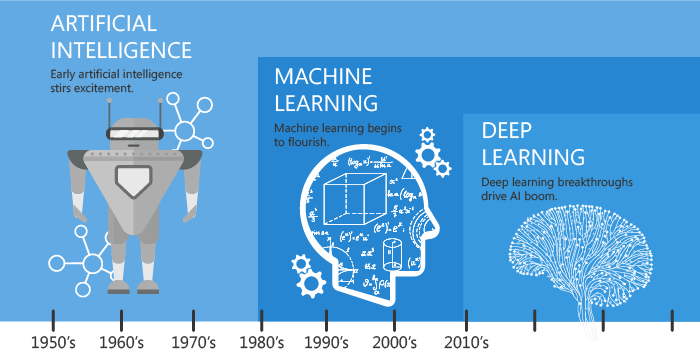
\includegraphics[scale=0.55]{sections/machine-learning/images/ki-ml-dl.png}
    \caption{Evolution von Künstlicher Intelligenz}
    \label{fig:kimldl-comparison}
\end{figure}
%https://miro.medium.com/max/700/0*jng0i9svVVe7L7sj

\subsubsection{KI - Künstliche Intelligenz}

Bereits in den 1950er erschien der Begriff ''Künstliche Intelligenz'', auf englisch ''Artificial Intelligence'', im Bereich Informatik, um Aufgaben zu lösen. Anfänglich noch mit dem Brettspiel "Dame" und einfachen Logikaufgaben. Jedoch kann es sich bei einer KI nur um eine programmierte Regel handeln, da man nur erwartet, dass sich die KI in gewissen Situationen auf eine bestimmte Art und Weise reagiert. Daher beschreibt es Programme, die humane Funktionen, imitieren und gibt nicht an mit welcher Technik das Problem gelöst wird. 

\subsubsection{ML - Machine Learning}

Der Unterschied zur Künstlichen Intelligenz liegt beim Vorgang des Lernens. Genau wie ein menschliches Gehirn muss ein Machine Learning Model mit Daten trainiert werden, mit welchen das Model dann gewisse Klassifizierungen, Clusterbildungen oder Regressionen durchführen kann. Über die Zeit verbessert sich die Präzision, da diese mit Zuwachs der eingespielten Daten wächst.

\subsubsection{DL - Deep Learning}

Sowie beim Machine Learning sind Deep Learning Algorithmen abhängig von antrainierten Daten und kann daher als Synonym oder Untergruppe vom Machine Learning gesehen werden. Jedoch kann ein DL Model wie ein Mensch noch nie davor gesehene spezielle Bilder kategorisieren und ist damit einem ML-Modell in vielen Hinsichten überlegen. 

Ohne Deep Learning würden die meisten modernen Assistenten nicht auf dem Niveau arbeiten wie erwartet, dabei handelt es sich bei Deep Learning um eine junge Technologie, die auf Neuronale Netzwerke basiert.

\paragraph{ML vs DL}

\subparagraph{Feature Extraction}

\begin{figure}[h]
    \centering
    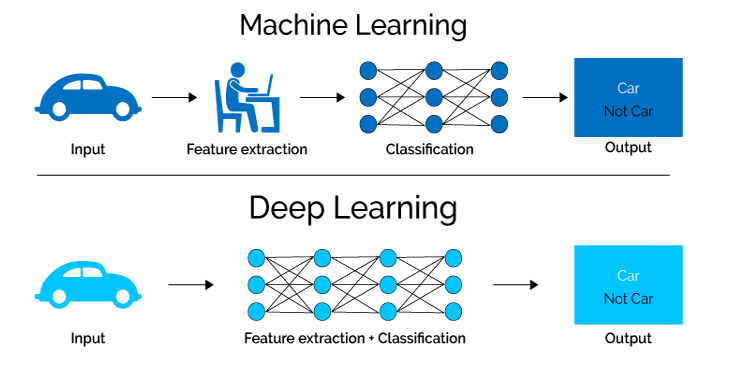
\includegraphics[scale=0.6]{sections/machine-learning/images/MLvsDL.png}
    \caption{Feature Extraction, ML vs DL}
    \label{fig:kimldl-comparison}
\end{figure}

Bevor ein ML-Modell mit der eigentlichen Verarbeitung beginnen kann, müssen die Rohdaten einer sogenannten "Feature Extraction" unterlaufen, welche die gegebenen Daten abstrakt darstellt. Dieser Prozess ist oft sehr kompliziert und beansprucht eine lange Zeit, außerdem ist hier eine Person notwendig, die sich in dem gegebenen Bereich auskennt.

Im Kontrast dazu gibt es Neuronale Netzwerke, welche den Feature Extraction Schritt übernehmen und selbstständig Rohdaten verarbeitet. Über mehrere Schichten werden bestimmte Merkmale hierarchisch definiert und später zum Beispiel zur Kategorisierung genutzt, hierbei erhöht sich die Genauigkeit der Extrahierung schon während des Antrainierens.

\subparagraph{Welches Verfahren ist sinvoller?}

In Bereichen, wo bereits strukturierte Daten vorhanden sind, bietet sind ein ML-Modell an, ein gutes Beispiel dafür ist die Erstellung von Vorhersehung von Ereignissen. Außerdem benötigt man keine große Menge an Daten, um genaue Ergebnise zu bekommen.

Stehen keine bereits vorpreperierte Daten zur Verfügung, wäre ein DL-Modell die bessere Lösung, aber dies auch nur wenn man eine große Menge an Daten hat.

\subsection{Arten}

Der wichtigste und komplizierteste Teil beim maschinellen Lernen ist die Kunst, einem Computer das selbstständige Lernen beizubringen, dabei orientiert man sich am Lernprozess eines Menschen. Dazu existieren eine Vielzahl an Ansätzen und zu den bekanntesten gehören:

\begin{itemize}
      \item Supervised Learning
      \item Unsupervised Learning
      \item Reinforcement Learning
\end{itemize}

Um diese Ansätze nachvollziehen zu können, muss man zuerst die menschliche Intelligenz verstehen oder genauer gesagt, die Frage ''Wie lernt das menschliche Gehirn?''.

\subsubsection{Menschliche Ursprünge vom Machine Learning}

Bereits als Fötus entwickeln sich Neuronen, die sich über die Zeit verknüpfen und gemeinsam ein Netzwerk bilden, welches dem Körper Anweisungen übermittelt. Daher kommt ein Neugeborenes mit etwa 100 Milliarden Neuronen auf die Welt, die zur Zeit der Geburt nur schwach miteinander verbunden sind. Mithilfe des Lernens werden diese Verbindungen gestärkt, und das Kind kann Vorgehensweisen besser verstehen und neue Erkenntnisse gewinnen, damit steigen zusätzlich auch das Gewicht und die Größe des Gehirnes. \cite{LANP}

Jedoch verschwinden diese Verbindungen, falls sie nicht aufgefrischt werden und Informationen in Vergessenheit verfallen. Weitere Faktoren könnten der Alterungsprozess oder eine neurologische Krankheit sein, die das Phänomen erklären, dass man im höheren Alter Probleme beim Erlernen von Neuem hat. \cite{GENTW}

\begin{figure}[H]
      \centering
      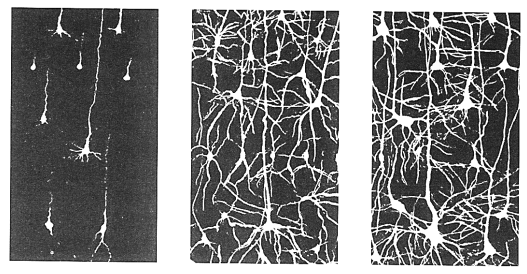
\includegraphics[scale=0.8]{sections/machine-learning/images/neuronale-netze.png}
      \caption{Vernetzungen nach der Geburt, nach 3 Monaten und nach 15 Monaten}
\end{figure}
%https://www.uni-wuerzburg.de/fileadmin/06000060/04_Fort-_und_Weiterbildungen_Lehrkraefte/Herbsttagungen/Herbsttagung_2016/20161006_WS_04_Neurobiologie.pdf

Neue Informationen verbinden bereits bestehende Neuronen und altes Wissen wird erneuert. Außerdem wird mit oftmaligem Wiederholen das Netzwerk dichter, und man kann das Erlernte leichter abrufen, zugleich werden die neuen Informationen mit dem bereits existierenden Vorwissen besser kombiniert. \cite{LANP}

\subsubsection{Supervised Learning}

An einen Algorithmus werden gruppierte Daten übergeben, die neben einer Gruppe noch mehrere Merkmale beinhalten, um danach neue Datensätze zu klassifizieren oder zu regredieren. Die Bezeichnung ''Supervised'' (im Deutschen ''Überwachtes'') kommt daher, dass die Gruppen bereits vordefiniert sind und das Programm nicht selber welche erstellen muss. \cite{SL:online}

\begin{table}[H]
      \centering
      \resizebox{.7\textwidth}{!}{
            \begin{tabular}{|l|l|l|l|}
                  \hline
                  \textbf{Farbe} & \textbf{Form} & \textbf{Geschmack} & \textbf{Frucht} \\ \hline
                  rot            & herzförmig    & süß                & Erdbeere        \\ \hline
                  gelb           & oval          & säuerlich          & Zitrone         \\ \hline
                  rot            & rund          & süß                & Apfel           \\ \hline
                  grün           & rund          & säuerlich          & Apfel           \\ \hline
            \end{tabular}}
      \caption{Beispiel für gruppierte Daten als Tabelle; Merkmale: Farbe, Form, Geschmack; Gruppe: Frucht}
      \label{tbl:fruit-data}
\end{table}

Diese Art von Lernen kann man in zwei Typen aufteilen:

\begin{itemize}
      \item Klassifizierung
      \item Regression
\end{itemize}

\paragraph{Klassifizierungs} Probleme verwenden Algorithmen, um Daten einer bestimmten Kategorie zuzuteilen. Oft gibt es nur zwei Kategorien wie zum Beispiel Hund/Katze oder Ja/Nein, jedoch gibt es auch Fälle, wo eine Vorhersage mit einer Wahrscheinlichkeit zwischen 0 und 1 getroffen wird. Weiteres gibt es auch Situationen, wo zwischen einer großen Menge an Kategorien ausgewählt wird, zum Beispiel bei der Erkennung von handschriftlichen Ziffern, in diesem Beispiel würde es zehn Möglichkeiten geben.

\begin{figure}[H]
      \centering
      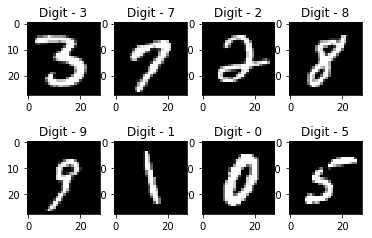
\includegraphics{sections/machine-learning/images/0_8-vKSQnZvKbtKXKy.png}
      \caption{Beispiel für eine Klassifizierung von handschriftlichen Ziffern}
      \label{ziffern}
\end{figure}
% https://aleenamishra10.medium.com/handwritten-digit-recognition-using-machine-learning-f6a08761ff83

Zu diesen ''überwachten'' Algorithmen gehören Lineare Diskriminanzanalysen, Support Vector Machines (SVM), Random Forests und Entscheidungsbäume.\cite{SL:online}

\subparagraph{Entscheidungsbäume} (Decision Trees) sind eine hierarchische Abfolge von Bedingungen und sind vergleichbar mit verschachtelten if/else-Statements. Dabei beginnt der Entscheidungsbaum mit einer Bedingung, die auch als ''Root-Node'' bezeichnet wird, worauf im Normalfall weitere Bedingungen folgen. Die Blätter dieser Pfade spiegeln die Gruppen oder Klassifizierungen wieder und sind nur über mehrere Pfade erreichbar.

Jedoch haben Entscheidungsbäume das Problem, dass sie sehr gut mit den antrainierten Daten arbeiten und weniger genau mit neuen Daten (Overfitting \ref{overfitting}). Um diese Genauigkeit zu verbessern, kann man zum Beispiel über Hyperparameter die maximale Länge eines Pfades setzen, wodurch die Bedingungen verallgemeinert werden.

\begin{figure}[H]
      \centering
      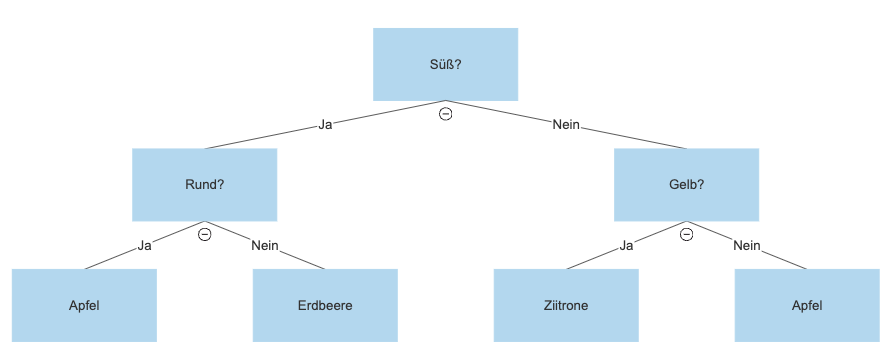
\includegraphics[scale=0.5]{sections/machine-learning/images/decision-tree.png}
      \caption{Decision Tree an dem Beispiel von Tabelle \ref{tbl:fruit-data}}
\end{figure}

In diesem Beispiel sieht dieser Entscheidungsbaum noch sehr lesbar aus, jedoch ändert sich dies, wenn Entscheidungen dargestellt werden, bei denen es auf die Nachkommastelle ankommt und wenn die Kategorien sehr schwer differenzierbar sind. Bei dem Supervised Learning erstellt das Programm selbstständig einen Entscheidungsbaum, indem es Muster oder Zusammenhänge findet und analysiert. Nach vielem Lernen kann dieser Entscheidungsbaum optimiert werden und unnötige Verbindungen können entfernt werden.

Fasst man mehrere Entscheidungsbäume zusammen, entsteht ein Random Forest, wobei jeder Entscheidungsbaum nur bestimmte Spalten/Merkmale zugeteilt bekommt. Soll ein neuer Datensatz kategorisiert werden, entscheidet die Mehrheit jener Ergebnisse der Entscheidungsbäume, zu welcher Gruppe dieser Datensatz dazugehört.

\paragraph{Regressionen,} Erstellung einer kontinuierlichen Funktion mithilfe von Werten, die auf oder nahe an der Funktion liegen, sind hilfreich, wenn anstatt diskreten kontinuierlichen Werte, wie zum Beispiel die Größe einer Person, festgestellt werden sollen. Dazu gehören lineare Regressionen und polynominale Regression.

\subsubsection{Unsupervised Learning}

Beim Unsupervised Learning oder unüberwachtes Lernen werden Verbindungen ohne genauere Informationen über den Testdatensatz erzeugt. Dabei muss das Programm selbst Gruppen definieren und dann die übergebenen Daten in diese Gruppen zuordnen. \cite{SL:online}

\paragraph{Clustering} gehört zu den beliebtesten Varianten, um selbstständig Gruppen zu erstellen. Dabei wird jeder Datensatz als Punkt in ein Koordinatensystem mit beliebig vielen Dimensionen eingetragen. Eine Achse stellt ein Attribut dar und je nach Ausprägung ist der Punkt mehr oder weniger vom Ursprung entfernt.

\begin{figure}[H]
      \centering
      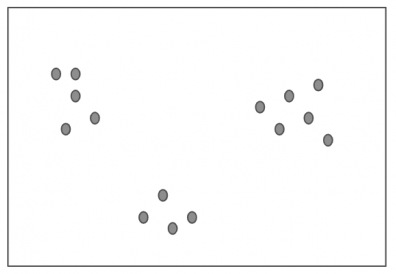
\includegraphics[scale=0.8]{sections/machine-learning/images/unclustered-data.png}
      \caption{Unkategorisierte Daten}
      \label{fig:unclustered-data}
\end{figure}
%https://datascience.eu/de/maschinelles-lernen/clustering-algorithmen-und-ihre-bedeutung-beim-maschinellen-lernen-2/

Auch für das menschliche Auge ist es möglich, dieses Beispiel (Abbildung \ref{fig:unclustered-data}) in Haufen oder Klumpen zusammenzufassen, genau das gleiche macht ein Programm mit Clustern. Die Interpretation dieser Gruppen muss jedoch wieder durch Menschen erfolgen, da ein Computer nicht im Stande dazu ist, diese Cluster einer Kategorie zuzuteilen.

Diese Vorgehensweise wird oft in sehr komplizierte Einsatzbereiche genutzt und daher ist es sehr schwer, differenzierbare Cluster zu erstellen. Der Prozess, solche Cluster zu definieren, basiert darauf, die Punkte so zu gruppieren, dass der Abstand in diesem Cluster klein ist und zu anderen Clustern groß.

\begin{figure}[H]
      \centering
      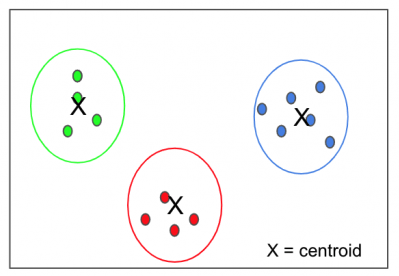
\includegraphics[scale=0.8]{sections/machine-learning/images/clustered-data.png}
      \caption{Kategorisierte Daten}
      \label{fig:clustered-data}
\end{figure}

\subsubsection{Reinforcement Learning}

Das Reinforcement Learning oder das beschränkte/verstärkte Lernen wird oft mit dem Konzept ''Learning by doing'' verglichen, da es sich weniger auf das Ergebnis fokussiert und mehr auf Aktionen oder Vorgängen. Ein Beispiel für diese Vorgehensweise aus der Sicht eines Schülers ist das Üben vor einer Matheschularbeit. Wird während dem Üben ein Fehler gemacht, merkt man sich das Problem und passt sein Verhalten / seinen Rechenweg so an, dass dieser Fehler nicht mehr vorkommt. Diesen Vorgang nennt man auch negative Verstärkung. \cite{SL:online}

Dahingegen führen richtige Ergebnisse oder erwartete Reaktionen zu positiven Verstärkungen und man versucht dieses Verhalten zu wiederholen.

Durch negative und positive Verstärkungen wird das Verhalten verbessert, um den besten Weg zum Ziel zu finden. Bei komplexen Systemen kann dies selbstständig vom Programm gemacht werden, jedoch bei simpleren kann es geschehen, dass ein unnötig komplizierter Weg gefunden wird. In diesen Fällen schaut ein Supervisor dem Programm ''über die Schulter''.

\subsection{Optical Character Recognition}

In den meisten Fällen erfolgt eine Eingabe über eine Tastatur, jedoch ist dies manchmal weder die beste noch effizienteste Art, Text einzulesen. Mithilfe von \gls{ocr} ist ein automatisiertes Einlesen und Verarbeiten von handschriftlichen oder gedruckten Text möglich und das schon bereits in den 1950er. Am Anfang noch um Verkaufsberichte in Lochkarten zu konvertieren, damit ein Computer mit den Verkaufsdaten arbeiten kann \cite{OCR:online}.

Im Bereich von \gls{ocr} sind bereits momentan gute und präzise Resultate mit \glsfirst{ml} erwartbar, jedoch wie bei allen anderen Problem ist es verbesserbar. Um einen großen Fortschritt zu erreichen, würde die Nutzung von Deep Learning verpflichtend sein, dies ist jedoch in den meisten Situationen nicht notwendig.

Die Präzision hängt von vielen Attributen ab, daher kann ein eingescannter Text viel besser verarbeitet werden, als ein in der Freien geschossenes Bild mit dem Fokus auf ein Straßenzeichen \cite{OCR2:online}. 

\begin{itemize}
    \item Textdichte 
    
    Es macht einen Unterschied wie viel Text sich auf einer Fläche oder einem Bild befindet, denn es ist in gewissen Situationen leichter Text auszulesen, wenn dieser nur spärlich vorkommt. 
    \item Struktur
    
    Wenn man eine klare Struktur erkennt, zum Beispiel in Tabellen oder in Zeilen, kann man ein besseres Ergebnis erwarten, daher ist es auch wichtig, dass man vor dem Auslese-Prozess das übergebene Bild aufbereitet und als Beispiel die Rotation ändert. 
    \item Schriftart
    
    Handgeschriebene Texte oder ''laute'' Schriftarten sind im Gegensatz zu einfachen und gedruckten viel komplizierter, da sie kaum strukturiert sind. Außerdem könnten Buchstaben Ähnlichkeiten aufweisen, was später zu Verwechslungen führen kann.
    \item Buchstaben
    
    Sprachen wie Arabisch, Chinesisch, Russisch oder Japanisch benutzen im Gegensatz zu Deutsch ein anderes Alphabet, dabei kann es zu ähnlichen Buchstaben und Vertauschungen kommen, daher sinkt die Präzision in Texten mit mehreren Sprachen. Dies kann auch der Fall sein, wenn mathematische Formeln vorkommen.

    \begin{table}[H]
        \centering
        \begin{tabular}{|l|l|}
            \hline
            Kyrillisches Alphabet & Ähnelt dem Buchstaben im lateinischem Alphabet  \\ \hline
            \foreignlanguage{russian}{r} & p \\ \hline
            \foreignlanguage{russian}{V} & B \\ \hline
            \foreignlanguage{russian}{N} & H \\ \hline
            \foreignlanguage{russian}{U} & y \\ \hline
            \foreignlanguage{russian}{S} & C \\ \hline
        \end{tabular}
        \caption{Ähnlichkeiten zwischen Buchstaben im Lateinischem und Kyrillischem Alphabet}
    \end{table}
    \item Platzierung
    
    Zentrierte Texte erlauben ein besseres Auslesen, als abgeschnittene oder verstreute Wörter.
\end{itemize}

Die Texterkennung ist generell in zwei Phasen aufgeteilt:

\begin{itemize}
    \item Text Detection
    \item Text Recognition
\end{itemize}

\subsubsection{Text detection} ist der Prozess, indem in einem Bild oder einer PDF erkannt wird, wo sich Text befindet. Beim Resultat handelt es sich um Bounding Boxen, diese schließen einen Textblock (Wort, Buchstabe oder Paragraph) ein, dabei werden die genauen Koordinaten der Eckpunkte zurückgegeben. Diese werden später genutzt, um zur Visualisierung Boxen auf dem Bild oder der PDF aufzuzeichnen. Dieser Prozess wird auch in der Objekterkennung genutzt.

\begin{figure}[H]
    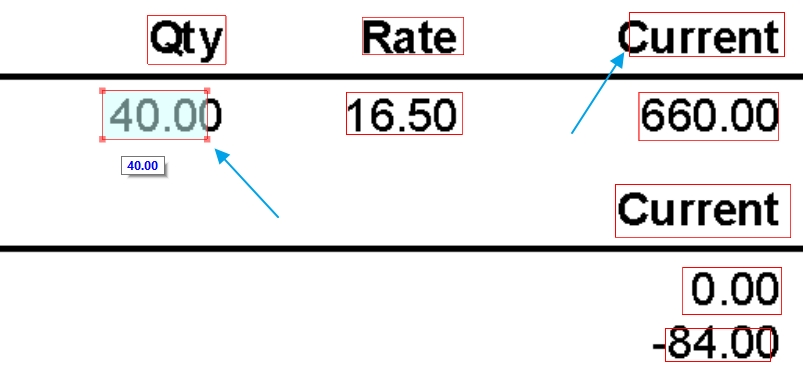
\includegraphics[scale=0.5]{sections/machine-learning/images/bounding-boxes.png}
    \caption{Bounding Boxes Beispiel}
    \label{fig:bounding-boxes}
\end{figure}

Die Erkennung kann entweder mittels der auf Regionen basierenden oder Textur basierenden Methode durchgeführt werden.

Bei der Regionen basierten Methode, werden Pixel verbunden und als Zeichenkandidat markiert, welche später mehrmals gruppiert werden und schlussendlich Wörter oder Textzeilen bilden. Dabei kommt es auf die geometrischen Eigenschaften an, wo es zu Fehlern beim Gruppieren kommen könnte. Wie man bei Abbildung \ref{fig:bounding-boxes} sehen kann, wurde der Buchstabe ''C'' im Wort ''Custom'' oder die letzte Nachkommastelle bei ''40.00'' nicht ganz als Teil des Wortes oder der Zahl erkannt.

Mit dem \Gls{swt} wird jedem Pixel eine Strichbreite zugeteilt, indem zwei Kanten gefunden werden mit der gleichen Richtung modulo 180°. Die Entfernung dieser zwei Kanten werden in den Kantenpixeln und alle unterliegenden Pixeln als Strichbreite gespeichert und alle Zusammenliegeden, gleich breite Pixel werden zu einem Zeichenkandidaten gruppiert. Danach werden alle benachbarten Zeichenkandidaten untersucht und zu einem Wort gruppiert, falls das mittelwertige Strichbreite-Verhältnis nicht über 2 liegt. Außerdem wird die Höhe und Farbe des Zeichenkandidaten berücksichtigt. Dies kann auch der Grund sein, wieso bei Abbildung \ref{fig:bounding-boxes} das Minuszeichen bei ''-84.00'' nicht zur Zahl hinzugefügt wird, das Minuszeichen ist signifikant niedriger als der Rest der Zahl. \cite{SWT:online}

\begin{figure}[H]
    \centering
    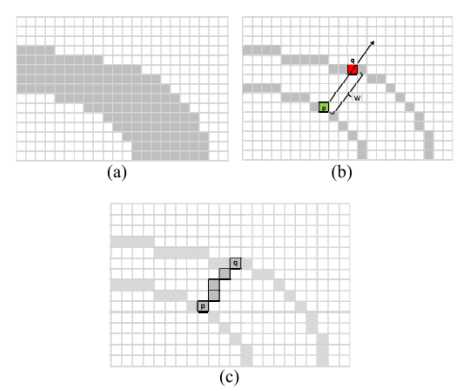
\includegraphics[scale=0.7]{sections/machine-learning/images/SWT.png}
    \caption{Die Kanten des Striches (a) werden solange verglichen, bis zwei gefunden werden mit der mit der gleichen Richtung (b). Alle unterliegenden Pixel erhalten die Strichbreite der Entfernung zwischen der Start- und Endkante (c).}
\end{figure}

Textur basierte Methoden unterteilen das Bild in Fester, dessen Höhe wird später mit der geschätzten Textgröße verglichen. Dabei kann es ebenfalls zu Erkennungsfehlern kommen.

Die Mischung dieser beiden Methoden gewann im Jahr 2011 den ICDAR-Wettbewerb \ref*{ICDAR} mit einem F-Score von 71.28\%. Hierbei hat Chunghoon Kim den Vorschlag gegeben, dass als erstes Blöcke  mit dem \Gls{mser} Verfahren extrahiert und danach benachbarte Blöcke gruppiert werden, falls die Farbe und Größe sich ähnelt. Jedoch werden mit diesem Verfahren, ebenfalls eine große Menge an false-postive Blöcken erkannt. Um diese Anzahl zu verringern wird eine ähnlich Idee zur \gls{swt} verwendet. \cite{SWT:online}

\paragraph{Wettbewerbe}\label{ICDAR} sind ein großer Grund für die Fortschritte in der Texterkennung und im Rahmen des zwei-jährlich stattfindenden \Gls{icdar} Wettbewerbs wurden alle oben genannten Ideen verglichen \cite{ICDAR:online}.

\subsubsection{Text Recognition} ist genau wie bei der Erkennung von Text in zwei Möglichkeiten unterteilt: Regionen basierend und Textur basierend. 

Die von \gls{mser} generierten und normalisierten Blöcke werden je nach der Orientierung in ein seerates Bild extrahiert. Dabei sind acht Orientierung möglich, welche mit ein Gaußschem Filter bearbeitet werden und auf ein 5 x 5 Bild komprimiert wurden. Mit diesen 5 x 5 x 8 = 200 dimensionalen Vektoren werden, dann die bereits erkannten Blöcke klassifiziert. \cite{SWT:online}


\section{Praxis: Python}

\subsection{Python als Progrmmiersprache}

Nach dem Scheitern seiner ersten Programmiersprache, entwickelte Guido van Rossum die Sprache Python, dabei wollte er alle Fehler, die er beim Entwickeln von ABC gefunden hat, verbessern. Daher basieren auch die Stukturen und Konventionen von Python auf Unix, ohne an Unix gebunden zu sein. 

Python unterscheidet sich in vielen Punkten zu anderen Sprachen, unteranderem dass sie viel Wert auf Lesbarkeit gibt. Die auffälliste davon ist, dass Einrückungen Codeblöcke unterteilt anstatt eine Art von Klammern. Dafür gibt es zwei Gründe:

\begin{itemize}
    \item Es macht den Code kürzer und er wirkt nicht unnötig ausgeschmückt, daher braucht man eine kürzere Aufmerksamkeitsspanne um den Sinn einer Codestelle nachvollziehen zu können.
    \item Die Stuktur des Codes ist vereinhaltlicht, was es einfacher macht Projekte von anderen zu verstehen.
\end{itemize}

Außerdem werden dem Entwickler in vielen Entscheidungen leichter gemacht, da unnötige Möglichkeiten entfernt wurden, das heißt, dass es meisten nur eine offensichtliche Art und Weise gibt, etwas zu implementieren. Dazu kommt noch die Nutzung von Spezialzeichen, es werden nur Zeichen unterstützt, die den meisten bereits bekannt sind und dessen Operation Sinn machen. \cite{PythonGVR:online}

Dies beantwortet jedoch nicht die Frage ''Wieso ist Python die beliebteste Sprache für \gls{ml}?''. Die Antwort darauf ist, dass die Sprache nicht nur triviale Aufgaben bereits vorimplementiert, sonder auch, dass die meisten ML Funktionen in Python Libraries zusammengefasst sind. Daher muss man als Neuanfänger oder Fortgeschrittener keine bereits gelösten Probleme von Grund auf noch einmal angehen.

\subsection{Notebooks}

Da es bei \gls{ml} es öfters dazu kommt, dass bestimmte Codeblöcke oft wiederholt ausgeführt werden, kann man mit Hilfe von Notebooks diese einzelen ausführen. Zum Beispiel beim Analysieren eines Datensatzes oder schnell kleine Änderung am geplanten Vorgehen vorzunehemen.

Diese Codeblöcke können entweder Code, Texte oder Grafiken beinhalten, diese werden fortlaufend mit einer Nummer versehen und die Ausgabe/Grafik erscheint direkt unter dem Code.

\begin{figure}
    \centering
    \includegraphics{}
\end{figure}

%\begin{spacing}{1}
%	\chapter{Cloud Computing}
%\end{spacing}
%\setauthor{Moritz Polleichtner}

\section{Theorie}

\subsection{Was ist Cloud Computing?}

\begin{figure}[h]
    \centering
    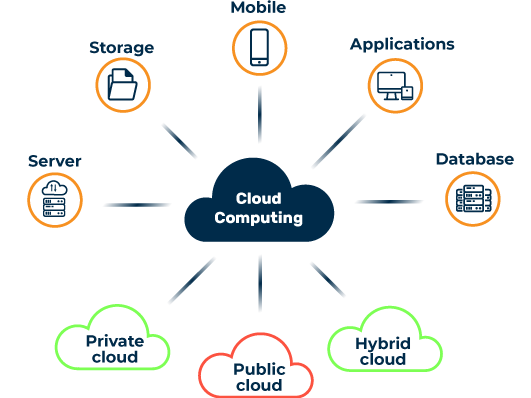
\includegraphics[scale=0.9]{sections/cloud-computing/images/cc.png}
    \caption{CC-Overview}
    \label{fig:kimldl-comparison}
\end{figure}

Cloud Computing ist ein Modell, bei dem virtueller Speicher, jegliche Art von Server, Anwendungen usw. nicht physisch, sondern rein über das Internet bereitgestellt werden. Diese werden in der Regel nach Bedarf als Teil eines As-a-Service-Modells angeboten. Üblicherweise wird dieses Modell in Verbindung mit nutzungsbasierter Bezahlung offeriert. Mithilfe der Cloud werden lokale Rechenzentren und interne Systeme mit virtuellen Rechen-, Netzwerk- und Speicherressourcen ausgetauscht. Im Normalfall werden diese Ressourcen von externen Anbietern bereitgestellt. Statt selbst breit gefächerte Rechen- und Speicherressourcen aufzustellen und nebenbei auch noch zu warten, wird eine Vielzahl dieser Aufgaben von einem Cloudservice-Anbieter übernommen.

\subsection{Vorteile von Cloud Computing}

Oft fallen, in Verbindung mit dem Thema Cloud Computing, Stichwörter wie „flexibel“ oder „agil“, das liegt daran, dass gerade in heutigen Zeiten marktseitige und auch technologische Veränderungen schnell und oft vorgenommen werden und deswegen Unternehmen oftmals nicht Schritt halten können. Deshalb betreiben viele Unternehmen sogenanntes Outsourcing, um nicht selbst für die Rechenleistung ihrer eigenen Dienste verantwortlich zu sein. Skalierbarkeit spielt hierbei eine große Rolle, zum Beispiel: je mehr Zugriffe auf einen Webshop, desto mehr Ressourcen müssen im Hintergrund hochgefahren werden, um eine fehlerfrei Nutzung zu garantieren.

Auch die Usability ist simpler bei cloudbasierten Prozessen, da viele dieser Prozesse in den Hintergrund verschoben und von den Cloud Service-Anbietern übernommen werden. Der Aufwand für Wartung, Beschaffung, usw. für Rechenzentren entfällt weitgehend. Somit kann man im Bereich Energie- und Erhaltungskosten einsparen. Im Allgemeinen werden die Kosten für solche Dienste je nach Vereinbarung nutzungsabhängig vereinbart. Im Normalfall fallen diese Kosten monatlich oder jährlich an, wobei diese verhältnismäßig kleiner als die von On-Premise Lösungen sind.

Ebenfalls ein wichtiges Stichwort hier ist Datenkonsistenz. Im Fall von komplexen Prozessen ist die Konsistenz der Daten ein wesentlicher Punkt, um drastische Probleme zu verhindern. Gerade bei dezentraler Speicherung und Verarbeitung der Daten, ist die Synchronität sehr wichtig. Bei Cloud Computing ist dieses Risiko minimiert, da im Normalfall die Daten, auch bei Zugriff von unterschiedlichen Schnittstellen, synchron sind.

\subsection{Hindernisse für den Einsatz einer Cloud}

Da es sich beim Cloud Computing um ein neues Modell handelt, besteht eine gewisse Unsicherheit, wie man auf allen Ebenen eine solide Sicherheit erreichen kann. Deshalb wird die Fähigkeit der Cloud, den Datenschutzbestimmungen gerecht zu werden, in Frage gestellt. Das Grundprinzip der Cloud sieht eine dauerhafte Verfügbarkeit vor und gerade diese Verfügbarkeit kann auch ein großer Nachteil sein. Erst durch den offenen Zugang zu den zur Verfügungen gestellten Rechenleistung und anderen Ressourcen, entfaltet das CC-Model sein volles Potenzial. 

Heutzutage müssen Anwendungen dauerhaft erreichbar sein und hierbei kann sich die Abhängigkeit von einem Cloud Service Provider negativ auf dauerhafte Konnektivität auswirken. Im Fall eines Ausfalls oder von Aussetzern müssen Notfallpläne- und oder Ressourcen gestartet werden um, zum Beispiel Datenverlust zu verhindern, was im Allgemeinen, zu fatalen Fehlern führen kann.

%https://www.ias.uni-stuttgart.de/service/begriffslexikon/bedeutung-der-interoperabilitaet-fuer-das-internet-der-dinge/
Die Interoperabilität und Übertragbarkeit von Informationen zwischen privaten und öffentlichen Clouds sind entscheidende Voraussetzungen für die breite Einführung von Cloud Computing in Unternehmen. Viele Unternehmen haben erhebliche Fortschritte bei der Standardisierung ihrer Prozesse, Daten und Systeme durch die Einführung von ERPs gemacht. Dieser Prozess wurde ermöglicht durch skalierbare Infrastrukturen, zur Schaffung einzelner Instanzen oder hochintegrierter Verbindungen zwischen Instanzen, um die Konsistenz von Stamm- und Bewegungsdaten zu verwalten und zuverlässige konsolidierte Informationen zu erzeugen.


\subsection{Cloud Computing Modelle}

\begin{figure}[h]
    \centering
    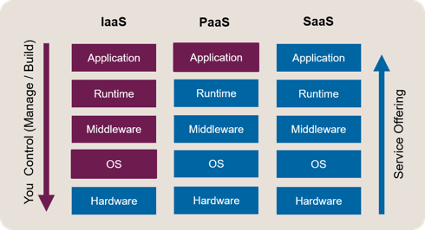
\includegraphics[scale=0.9]{sections/cloud-computing/images/models.png}
    \caption{Modelle}
\end{figure}

\subsubsection{Infrastructure as a Service (IaaS)}

Infrastructure as a Service stellt sowohl virtuelle und physische Server, als auch Netzwerk- und Speicherressourcen, nach Verlangen des Verbrauchers, zur Verfügung. Der Nutzer hat die völlige Kontrolle über Ressourcen, in Bezug auf Speicher und Rechenleistung. Die Auswahl des Betriebssystems wird ebenfalls dem Nutzer überlassen. Beispiele hierfür sind Amazon EC2-Cluster und Microsoft Azure.

\subsubsection{Platform as a Service (PaaS)}

Diese Form des Cloud Computing gibt dem Kunden die Möglichkeit, seine Anwendungen auf einer, vom Dienstleistungsgeber, gehosteten Plattform zu entwickeln, bereitzustellen und zu verwalten. Bei diesem Modell handhabt der Dienstleister sämtliche Ressourcen. Die Anwendung wird den potenziellen Nutzern über APIs zur Verfügung gestellt. Hierbei ist wichtig, dass der Nutzer keinerlei Einfluss über, die im Hintergrund laufenden, Ressourcen hat. Bekannte Beispiele hierfür sind Web-Hosting Dienste, wie etwa +Microsoft Azure Web und Amazon Web Services.

\subsubsection{Software as a Service (SaaS)}

Bei SaaS wird den Nutzern die Möglichkeit gegeben auf eine, vom Dienstleister in der Cloud Infrastruktur bereitgestellten Anwendung, zu zugreifen und zu benutzen. Benutzer können dann über eine webbasierte Schnittstelle, wie beispielsweise ftp und clientseitige Schnittstellen, darauf zugreifen. Jene Anwendungen werden gegen monatliche oder jährliche Zahlungen dem Benutzer bereitgestellt. Jedoch hat der Verbraucher keine bis wenig Kontrolle über im Hintergrund geregelte Ressourcen. Beispiele hierfür sind Microsoft Office 365, Microsoft Skype und Google Apps.

\subsection{Anwendungsfälle von Cloud Computing}

\begin{figure}[h]
    \centering
    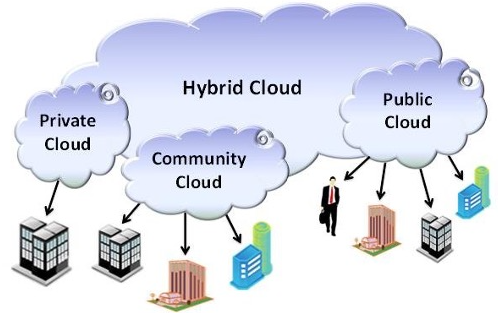
\includegraphics[scale=1]{sections/cloud-computing/images/cc-use-cases.png}
    \caption{Anwendungsfälle}
\end{figure}

\subsubsection{Private Cloud}

Dieses Bereitstellungsmodell wird vor allem in Unternehmen verwendet, das heißt diese Dienste sind nicht für die Öffentlichkeit zugänglich. Sie werden nur Unternehmensintern verwendet. Die Nutzer können standortunabhängig von diesen Cloud Computing Diensten Gebrauch machen, müssen aber Teil der gleichen Organisation sein. Die private Cloud ist die sicherste der Bereitstellungsmethoden. Der Grund dafür ist, dass Prozesse innerhalb des Unternehmens kontrolliert und verwaltet werden, ohne jegliche Leistungs- Sicherheitsbeschränkungen, die Dienste in der Public Cloud vielleicht benötigen. In der privaten Cloud ist es möglich, dass die fundamentale Infrastruktur der Cloud vom Unternehmen selbst, von Drittanbietern oder auch von Beiden verwaltet wird. Generell wird die Private Cloud in zwei unterschiedliche Arten unterteilt:

\begin{itemize}
    \item On-Premise Private Cloud
    \begin{sloppypar}
        Diese Art wird auch interne Cloud genannt. Sie bietet zusätzliche Sicherheit, dennoch kann sie in Größe und Skalierbarkeit stark eingeschränkt sein, da man selbst das Kapital für Hard- und Software, sowie Wartung und Instandhaltung aufbringen muss. Die interne Cloud eignet sich somit für Anwendungen, die die volle Kontrolle sämtlicher Ressourcen verlangen.
    \end{sloppypar}
    \item extern gehostete Private Cloud
    \begin{sloppypar} 
        Hier wird das Hosten der Cloud von einem Drittanbieter übernommen. Diese Anbieter fördern eine restriktive Cloud Computing-Umgebung mit vollständiger Vertraulichkeit. Diese Art der Private Cloud wird für Institutionen empfohlen, die das Kapital für eine interne Private Cloud nicht aufbringen können.
    \end{sloppypar} 
\end{itemize}

\subsubsection{Public Cloud}

Eine Public Cloud ist für die Öffentlichkeit zugänglich und kann von einem Unternehmen, einer staatlichen Einrichtung oder Organisation verwendet werden. Die Cloud ist jedoch im Besitz eines Drittanbieters. Hierbei greift der Nutzer über Schnittstellen auf die CC-Dienste des Cloud-Besitzers zu.

\subsubsection{Community Cloud}

In der Community Cloud wird die Infrastruktur einer Cloud von mehreren Unternehmen oder Institutionen mit ähnlichen oder gemeinsamen Zielen verwendet. Die Infrastruktur kann entweder von einer Organisation oder mehreren Organisationen verwaltet werden.

\subsubsection{Hybrid-Cloud}

Diese Variante ist eine Kombination aus einer oder mehreren privaten und öffentlichen Cloud, die aber als getrennte Einheiten fungieren. Diese Einheiten werden durch eine Protokollen und Standardisierungen verbunden. Dieses Modell wird hauptsächlich verwendet, wenn man die Vorteile der unterschiedlichen CC-Bereitstellungsoptionen kombinieren möchte. Beispielsweise, ein Unternehmen möchte die Datenspeicherung auf einer privaten Cloud realisieren, und andere Aufgaben mithilfe einer öffentlichen Cloud erledigen.

\subsubsection{Azure Cloud}

Microsoft Azure ist ein Cloud-Computing-Dienst von Microsoft. Azure bietet eine Reihe von Software as a Service (SaaS), Plattform as a Service (PaaS) und Infrastruktur as a Service (IaaS) Optionen, für die Bereitstellung von Anwendungen und Diensten, auf einer von Microsoft verwalteten Rechenzentrumsinfrastruktur an. Mit 50 Betriebsregionen bietet Azure mehr als jeder andere Cloud-Anbieter.



\section{Praxis: AI Builder}





Basierend auf Azure AI Cognitive Service ist AI Builder ein Tool, welches zum Erstellen und Trainieren von Modellen, ohne das Schreiben von Code dient. Die Integration mit Power Apps und Power Automate ist eine Funktion, die den Nutzern die Möglichkeit bietet, bestehende Geschäftsanwendungen zu erweitern, und zu verbessern.
Microsoft Power Plattform ist eine Low-Code-Plattform, die es Unternehmen bewilligt, Geschäftsprozesse zu automatisieren. Power Plattform umfasst drei Hauptprodukte: Power BI, PowerApps und Flow.
Mit dem AI Builder ist es möglich, auf einfache Weise Prozesse zu automatisieren und Ergebnisse vorherzusagen. AI Builder ist eine schlüsselfertige Lösung, die die Leistungsfähigkeit der künstlichen Intelligenz von Microsoft mit wenigen Mausklicks anwendbar macht. Mit dem AI Builder kann man Anwendungen Intelligenz beifügen, auch wenn Sie keine Programmier- oder Data-Science-Kenntnisse haben.

\subsection{Benutzerdefinierte Modelle}

Der erste Schritt bei der Erstellung eines KI-Modells besteht darin, festzustellen, ob für den Anwendungsfall bereits vorgefertigte oder bereits trainierte Modell vorhanden sind. Ist dies nicht der Fall, stehen in der Benutzeroberfläche des AI Builders fünf Modelle zur Verfügung:

\begin{enumerate}
    \item Category Classification
    \item Entity Extraction
    \item Form Processing
    \item Object Detection
    \item Prediction
\end{enumerate}

\begin{figure}[h]
    \centering
    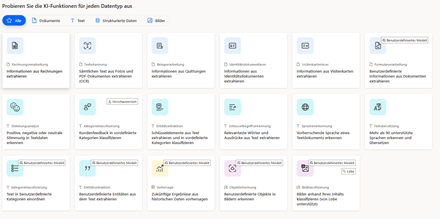
\includegraphics[scale=0.9]{sections/cloud-computing/images/ai-builder-models.png}
    \caption{AI-Builder Modelle}
    \label{fig:kimldl-comparison}
\end{figure}

\subsubsection{Category Classification}

Bei diesem Ansatz wird ein Modell verwendet beziehungsweise trainiert, um große Mengen an Textdaten, Dokumenten oder sonstige Textdatenquellen zu analysieren, und den Text zu klassifizieren. Besonders hilfreich ist dieses Modell, um Spam zu identifizieren, und entsprechend zu behandeln. Zuerst muss das Modell mit Trainingsdaten trainiert werden. Das Zeichenlimit für jede Textprobe liegt bei fünftausend Zeichen.

Die Analysen, die dieses Modell liefert, können auch als Input für andere KI-Lösungen verwendet werden. Wichtig hierbei ist, dass für jeden Tag mindestens zehn Textproben bereitgestellt werden, ansonsten sinkt die Wahrscheinlichkeit ein genaues Ergebnis zu erzielen.

\subsubsection{Entity Extraction}

Hier werden wichtige Textelemente identifiziert, ferner den definierten Kategorien zugeordnet. Die Ergebnisse werden dabei, entsprechend den Anforderungen, standardisiert und strukturiert. Auch hier werden wieder mindestens 10 Datensätze benötigt, um mit dem Trainieren des Modells beginnen zu können. Das Modell ist anpassbar, indem man neue Entitätstypen mit wenigen Trainingsdaten erstellt oder bestehende Entitätstypen modifiziert. Der Ai Builder verfügt über vorgefertigte Trainingsdaten, die zur Erweiterung der eigenen Trainingsdaten verwendet werden können.

\subsubsection{Form Processing}

Die Formularverarbeitung ist das KI-Modell, das Daten aus Formularen, auch aus Papier- oder PDF-Dokumenten, extrahiert. Es werden fünf Beispielformluare benötigt, ums es zu trainieren, die Felder eines Dokuments zuzuordnen und eine funktionierende Anwendung zu erstellen. Diese Lösung wird verwendet um Rechnungen und Aufträge zu erfassen. Beispielsweise ist es möglich, das Modell zu trainieren und einen Ablauf zu erstellen, der automatisch Schlüsselinformationen aus Bestelldokumenten erkennt, extrahiert und anschließend eine E-Mail an den zuständigen Mitarbeiter sendet.

Die empfohlenen Formate für die Eingabedaten sind .jpg, .png und .pdf. Die Gesamtgröße der, für das Training verwendeten, Dokumente, darf insgesamt 50 MB nicht überschreiten.

\subsubsection{Object Detection}

Die Objekterkennung wird verwendet, um Objekte auf Fotos oder Videos zu erkennen. Dieses Modell kann verwendet werden, um bestimmte Informationen von Produkten oder Maschinen zu erhalten. Ebenfalls hilfreich kann dieses Modell bei mobilen Anwendungen sein.

Für das Training werden mindestens 15 Fotos von jedem Objekt benötigt; je mehr Fotos, desto genauer ist das Modell.  Um eine korrekte Identifiezierung zu gewährleisten, sollten die Fotos möglichst verschiedene Hintergründen beinhalten. Ebenfalls empfehlenswert ist es, Fotos von Objekten aus diversen Entfernungen und Winkeln bereitzustellen. Es ist zu beachten, dass die Trainingsbilder im .jpg-, .bmp- oder png-Format vorliegen müssen und insgesamt 6 MB pro Training nicht überschreiten dürfen. Die Grenze von 256 x 256 Pixel soll jedoch nicht unterschritten werden.

\subsubsection{Prediction} 

Bei diesem Modell werden große Mengen an alten Daten analysiert, um darin Muster zu erkennen. Das gewonnene Wissen wird dann verwendet, um diese Muster in neuen Datensätzen zu erkennen, und Vorhersagen zu treffen.

Zum Trainieren des Modells werden mindestens 10 Zeilen mit historischen Werten, für jede Klasse der Datenspalte "Label", benötigt. Die Mindestanzahl der Zeilen für das Training liegt bei 50, aber ein Minimum von 1.000 Zeilen gewährleistet die erfolgreichsten Ergebnisse.

\subsection{AI-Builder in der Praxis}

Um den AI-Builder für den gewünschten Use-Case am effektivsten zu nutzen, hat sich das Diplomarbeitsteam dazu entschieden, das Modell des Form Processing zu verwenden. Der gewünschte Use-Case ist mehrere, im Vorhinein definierte Felder aus einer Eingangsrechnung, im PDF, zu extrahieren und anschließend zu markieren. 
Die untenstehende Abbildung dient zur veranschaulichung einer solchen Eingangsrechnung (Siehe Abbildung \ref{fig:example-invoice-figure}). Folgende Schritte sind ein wesentlicher Bestandteil, um ein Modell zu erstellen, dass auf spezielle Eingangsrechnungen trainiert ist:

\begin{enumerate}
    \item Zu extrahierende Felder definieren
    \item Trainingsdaten bereitstellen
    \item Trainingsdaten mit Tags versehen
    \item Modell trainieren und
    \item Modell veröffentlichen
\end{enumerate}

\begin{figure}[h]
    \centering
    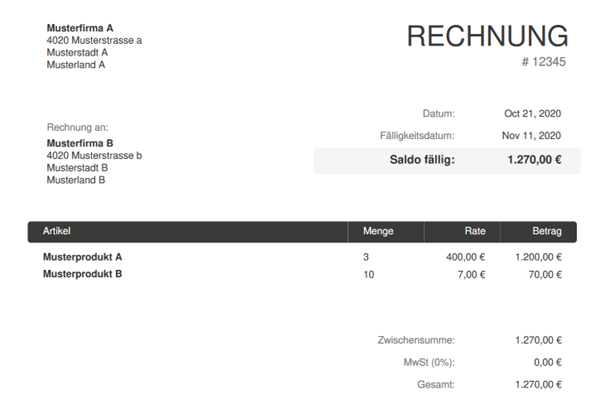
\includegraphics[scale=0.9]{sections/cloud-computing/images/example-invoice.png}
    \caption{Beispiel Eingansrechnung}
    \label{fig:example-invoice-figure}
\end{figure}

Zunächst ist es wichtig zu wissen, welche Felder man aus der ER extrahieren will. In der folgenden Abbildung wird gezeigt, welche Felder bei dieser Arbeit ausgewählt wurden. Jene Felder wurden nur zu Veranschaulichung der Fähigkeiten des AI-Builders ausgewählt:

\begin{figure}[h]
    \centering
    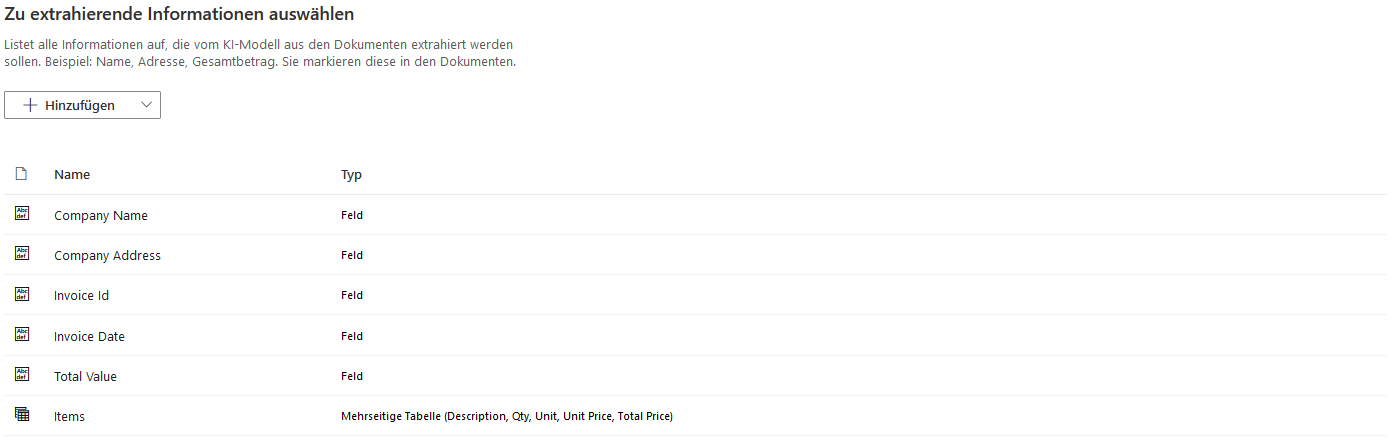
\includegraphics[scale=0.5]{sections/cloud-computing/images/ai-builder-fields.png}
    \caption{AI-Builder Felder}
    \label{fig:ai-builder-fields-figure}
\end{figure}

\begin{enumerate}
    \item Company Name
    \item Company Address
    \item Invoice Id
    \item Invoice Date
    \item Total Value
    \item Items (Mehrseitige Tabelle)
\end{enumerate}

\textbf{Items (Mehrseitige Tabelle)}: Diese Tabelle bietet ein experimentelles Feature, um tabellarische Daten aus einer, in der Rechnung vorhandenen Tabelle zu entnehmen, auch wenn sich die Tabelle über mehrere Seiten zieht. Diese Tabelle enthält wiederrum eigene Daten wie:

\label{enum:InvoiceItemsAttributs}
\begin{enumerate}
    \item Description
    \item Qty (Quantity)
    \item Unit
    \item Unit Price
    \item Total Price
\end{enumerate}


Um Daten für das Trainieren des Modells bereitzustellen, ist es notwendig mindestens fünf Beispieldokumente hochzuladen. Nichtsdestotrotz ist für eine hohe Genauigkeit des Modells, sprich wie sicher sich der Algorithmus ist, dass er das richtige Feld markiert hat, von Vorteil mehrere ähnliche Dokumente bereitzustellen. 
Um dem Algorithmus anzutrainieren, welche Felder in dem Dokument vorhanden sind, ist es relevant die Daten in dem Dokument händisch zu markieren, und die zuvor definierten Informationsfelder zu zuweisen. Siehe folgende Abbildung (\ref{fig:ai-builder-tagging-figure})

\begin{figure}[h]
    \centering
    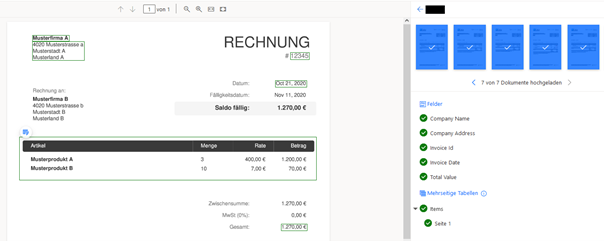
\includegraphics[scale=0.9]{sections/cloud-computing/images/ai-builder-tagging.png}
    \caption{AI-Builder Felder Tagging}
    \label{fig:ai-builder-tagging-figure}
\end{figure}

\section{Praxis: Power Atomate}

Power Automate ist ein Teil der Microsoft Power-Platform, mit der man Cloud-basierte Automatisierungsprozesse erstellen und verwalten kann. Der Benutzer hat Zugriff auf verschiedene Dienste von Microsoft und kann ohne oder wenig Code einen Workflow erstellen. Power Automate reagiert auf einen im Vorhinein definierten Trigger und führt eine Reihe von vordefinierten Schritten aus. Dieser Trigger kann eine neue E-Mail, ein neuer Datensatz im CRM eingefügt wird oder einfach die Erstellung eines neuen Dokuments im SharePoint sein. Somit ist es möglich auch ohne jegliche Vorkenntnisse oder fachspezifisches Wissen eine einfache Anwendung zu erstellen. Zum Beispiel kann beim Eingang einer E-Mail, die eine Kundenrechnung enthält, an den AI-Builder weitergegeben werden und dort mit einem vortrainierten Modell, die wichtigsten Daten herauslesen und dann erneut mit einer E-Mail versendet werden.

\subsection{Cloud Flow}
Da bei dieser Arbeit nur der Cloud Flow in Verwendung ist, wird hier nur auf diesen genauer eingegangen. Power Automate bietet hier drei verschiedene Arten von Cloud Flows an:

\begin{enumerate}
    \item Automated Flow
    \item Instant Flow
    \item Scheduled Flow
\end{enumerate}

\subsubsection{Automated Flow}
Dieser Flow wird ausgelöst, wenn eine gewünschte Kondition eintritt. Solche Trigger können, der Eingang einer E-Mail einer speziellen Person, eine Teams-Nachricht oder wenn ein Dokument in OneDrive geändert wird. Sogenannte Connectors werden verwendet, um eine Folge von Schritten zu bilden, um den gewünschten Effekt zu erzielen.

\subsubsection{Instant Flow}
Ein Instant Flow wird mit dem Klicken eines Buttons gestartet. Dieser Flow läuft sowohl auf Mobile als auch auf Desktop Devices. Er wird verwendet, um ein breites Spektrum von Aufgaben zu erledigen, wie die Beantragung einer Genehmigung via Teams oder SharePoint.

\subsubsection{Scheduled Flow}
Dieser Flow wird nach einem Zeitplan automatisiert und zu einem gewünschten Datum oder beliebiger Uhrzeit ausgeführt werden. Dieser Ablauf ist hilfreich, um zum Beispiel jeden Tag zur selben Uhrzeit einen Daten-Upload zu machen.

\subsubsection{Cloud Flow in der Praxis}
Die Diplomanden dieser Arbeit entschieden sich für einen Automated Flow, da dieser die gewünschte Funktion erfüllt. Wie bereits erwähnt, ist der Automated Flow ein Event-basierter Flow und wird durch das Erhalten einer E-Mail ausgelöst (Siehe Abbildung \ref{fig:flow-trigger}).

\begin{figure}[h]
    \centering
    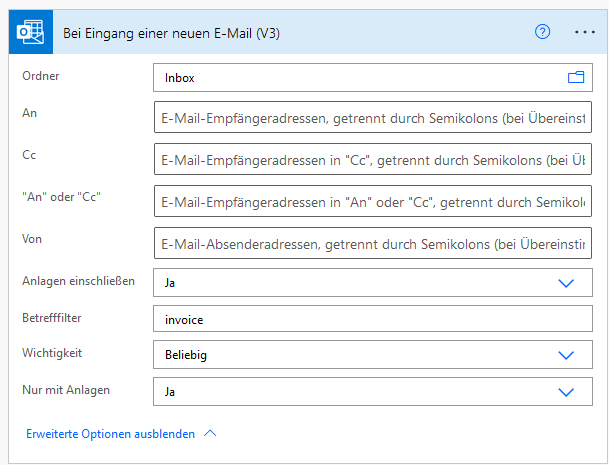
\includegraphics[scale=0.9]{sections/cloud-computing/images/power-automate-flow/trigger.png}
    \caption{Power Automate Flow Trigger}
    \label{fig:flow-trigger}
\end{figure}

Um alle Anlagen der E-Mail zu verarbeiten, wird eine Schleife um die nächsten Schritte gesetzt. Da es erlaubt ist mehrere Eingangsrechnungen in der E-Mail anzuhängen muss jeder Anhang einzeln verarveitet werden. Das zuvor definierte AI-Builder Modell extrahiert die notwendigen Information aus dem Dokument (Siehe Abbildung \ref{fig:ai-model-in-use}).

\begin{figure}[H]
    \centering
    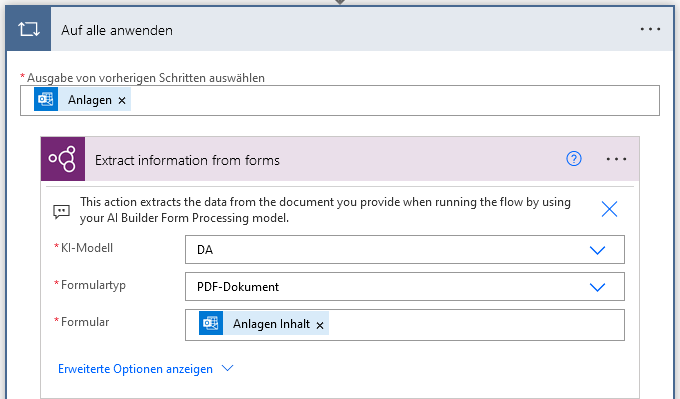
\includegraphics[scale=0.8]{sections/cloud-computing/images/power-automate-flow/ai-model-in-use.png}
    \caption{Verarbeitung des Dokuments}
    \label{fig:ai-model-in-use}
\end{figure}

Um die extrahierten Daten zu persistieren, wurde eine Dynamcis CRM Testumgebung aufgesetzt. Es wurden zwei Entitäten, Invoice und Invoice Items erstellt (\ref{fig:class-diagram}). Da die Entität Invoice Items von der Entität Invoice abhängig ist, muss die die Entität Invoice Items eigens gespeichert werden (Siehe Abbildung ... ).

\begin{figure}[h]
    \centering
    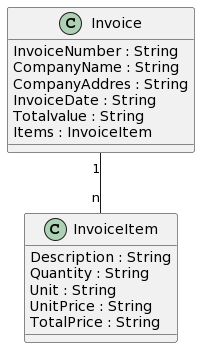
\includegraphics[scale=0.5]{sections/cloud-computing/images/power-automate-flow/cld.png}
    \caption{Klassendiagram Invoice}
    \label{fig:class-diagram}
\end{figure}

Um die Richtigkeit des Datenmodells zu sichern muss die Reihenfolge der Persistierung beachtet werden und alle Invoice Items abhängig von der dazugehörigen Invoice gemacht werden \ref{fig:persistence-entities}.

\begin{figure}[h]
    \centering
    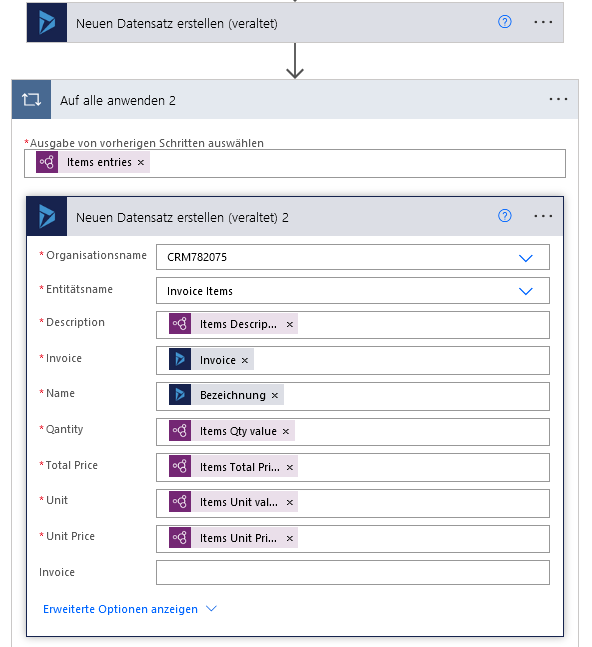
\includegraphics[scale=0.9]{sections/cloud-computing/images/power-automate-flow/insert2-dynamics-crm.png}
    \caption{Persistierung der Entitäten}
    \label{fig:persistence-entities}
\end{figure}

\ref{enum:InvoiceItemsAttributs}

\section{Praxis: Cognitive Services}

Die Azure Cognitive Services sind ein Teil der Cloud-basierten Dienste von Microsoft. Mithilfe von REST-APIs und Client-SDKs, ist es möglich kognitive Intelligenz in ihre Applikation einzubauen. Ein großer Vorteil ist, dass man dafür wenig bis keine Erfahrung im Bereich der künstlichen Intelligenz und Data Science benötigt. Die, in den Azure Cognitive Services, beinhaltete Sammlung an kognitive Funktionen ermöglicht es Lösungen zu erstellen, die menschliche Fähigkeiten wie sehen, sprechen und hören nachahmen.

\textbf{Kurzer Exkurs; REST-API, SDK:}

\begin{enumerate}
    \item \begin{figure}[h]
    \centering
    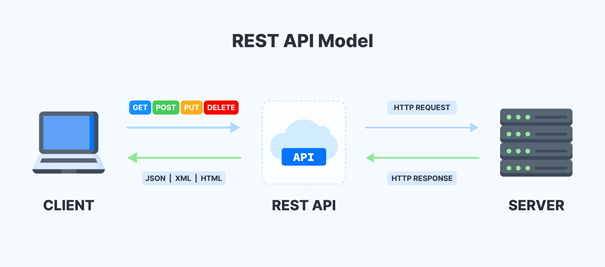
\includegraphics[scale=0.9]{sections/cloud-computing/images/rest-api.png}
    \caption{Funktionsweise von REST}
    \label{fig:ai-builder-tagging-figure}
\end{figure}

Stabile und interaktive Anwendungen setzten voraus, dass Programme untereinander barrierefrei kommunizieren können. Eine API, Application Programming Interface, definiert Regeln, die diese Kommunikation erleichtert. Unter diesen Programmen kann man entweder Softwarebibliotheken, ein Betriebssystem oder einen Webserver verstehen.
Der entscheidende Vorteil von API ist, dass das anfragende Programm keinerlei Informationen über das dahinterstehende System des Antwortgebers haben muss.

\textbf{REST-API}: Einer der bekanntesten Architekturen einer API ist REST. Representational State Transfer ist ein Stil für die Entwicklung von Anwendungen, die untereinander auf irgendeine Weise vernetzt sind. Es wird oft für die Entwicklung von Web-APIs verwendet.
Wichtig zu wissen ist, dass REST zustandslos ist. In diesem Kontext bedeutet zustandslos, dass Anfragen des Clients alle notwendigen Informationen für den Server besitzen muss. Der Client kann beispielsweise nicht davon ausgehen, dass sich der Server an die vorherigen Requests des Clients erinnern kann.
REST-APIs senden im Normalfall HTTP-Anfragen wie GET, POST, PUT, etc.

    \item Ein \textbf{Software Development Kit}, kurz SDK, ist eine Sammlung aus mehreren Tools, die von einem Hersteller einer Programmiersprache, eines Betriebssystems oder einer Hardwareplattform zur Verfügung gestellt werden. Diese Tools können Debugger, Frameworks oder eine Sammlung aus Codebibliotheken sein.
\end{enumerate}

\subsection{Cognitive Computing}

Cognitive Computing ist ein intelligentes System, das durch umfangreiches Lernen und zielgerichtetes Denken mit Menschen in ihrer natürlichen Form spricht und diese nachahmt. Cognitive Computing ist die dritte Ära der Informatik, und gleichzeitig hat Cognitive Computing sowohl in der Wissenschaft als auch in der Industrie breite Aufmerksamkeit auf sich gezogen. Die Kombination aus maschineller und menschlicher Intelligenz kann die komplexesten Probleme der Welt lösen. Die Verarbeitung natürlicher Sprache mit Sentimentanalyse, künstlicher Intelligenz (KI), maschinellem Lernen und neuronalen Netzen ist der Eckpfeiler von Cognitive-Computing-Prozessen, die Probleme wie Menschen lösen können. Heutzutage wenden fortschrittliche Technologien Cognitive Computing in vielen Bereichen an. Angesichts der heutigen Datenexplosion und der sich schnell ändernden Geschäftsumgebungen können kognitive Systeme intelligente, fließende und verbesserte Mensch-Maschine-Interaktionen effektiv angehen. Künstliche Intelligenz wird in vielen Anwendungen wie Alexa, dem Sprachassistenten von Amazon, Netflix und den Algorithmen von Amazon verwendet, um den nächsten Film oder Kauf vorzuschlagen. Einige Beispiele für persönliche Assistenten, die Cognitive Computing verwenden, sind Alexa, Siri, Google Assistant und Cortana. Die Weiterentwicklung dieser Technologie und ihre Übernahme im öffentlichen und privaten Sektor wird die Zukunft des Cognitive Computing aufgrund technologischer Entwicklungspfade und -trends stark beeinflussen. Kognitive Systeme müssen in Geschäfts- und breiten Anwendungen anpassungsfähig, interaktiv, iterativ, zustandsbehaftet und kontextbezogen sein. Zu den Anwendungen, die von solchen Technologien mit Cognitive Computing profitieren können, gehören Finanz- und Investmentfirmen, Gesundheitswesen und Veterinärmedizin, Reisen und Tourismus, Gesundheit und Wellness, Bildung und Lernen, Landwirtschaft, Kommunikations- und Netzwerktechnologie.

\subsection{Cognitive Computing und Cloud Computing}

Cloud Computing virtualisiert die Datenverarbeitung, den Speicher und die Bandbreite. Dadurch werden die Kosten für die Bereitstellung von Softwarediensten gesenkt und die Industrialisierung sowie die Förderung der Anwendung des Cognitive Computings unterstützt. Darüber hinaus bietet die hohe Rechen- und Speicherkapazität des Cloud Computing dynamische, flexible, virtuelle, gemeinsam genutzte und effiziente Rechenressourcendienste für das Cognitive Computing.

Nachdem die Big-Data-Analyse auf der CC-Plattform durchgeführt wurde, werden Technologien wie maschinelles Lernen eingesetzt, um Daten zu analysieren und die Ergebnisse in verschiedenen Bereichen anzuwenden. Die verschiedenen Kategorien von Informationen entsprechen unterschiedlichen Verarbeitungstechnologien. So entsprechen beispielsweise die wörtlichen Informationen der natürlichen Sprachverarbeitung und die bildlichen Informationen dem maschinellen Sehen. Der kognitive Dienst von IBM für Sprache und die kognitive Computing-Anwendung von Google legen den Schwerpunkt auf die Verwirklichung von gehirnähnlicher Wahrnehmung und Urteilsfähigkeit durch den Einsatz eines Cloud-Service-Modells, um präzise Entscheidungshilfen zu bieten. Cloud Computing und das Internet of Things (IoT) bieten eine Software- und Hardwarebasis für Cognitive Computing, während die Big-Data-Analyse Methoden und Denkweisen zur Entdeckung und Erkennung neuer Möglichkeiten und neuer Werte in Daten bereitstellt.



\begin{spacing}{1}
	\chapter{Ausgangslage}\label{chapter:tech}
\end{spacing}
\setauthor{Emina Sljivic}
\section{Ausgangssituation}

Als Mitglied der weltweiten Bechtle Gruppe stellt smartpoint IT consulting kundenspezifische Softwarelösungen im Bereich Office365, SharePoint und Dynamics 365/CRM bereit. Mit Standorten in Linz, Wien und Graz beschäftigt das Unternehmen über 100 Mitarbeiter, die mit laufenden Weiterbildungen immer auf dem neusten Stand der Technologie bleiben und dafür für das optimale Ergebnis sorgen.

Zusammen mit zahlreichen, namenhaften Unternehmen aus vielen unterschiedlichen Branchen werden seit 2007 Projekte gestartet, die noch bis heute laufen. Dabei bieten sie in allen Phasen der Projektentwicklung Unterstützung an, mit einer Spezialisierung auf Cloudlösungen. Dazu wird die User Experience und das Design auf keiner Weise vernachlässigt.

\begin{itemize}
    \item Beratung
    \item Konzeption
    \item Umsetzung
    \item Betreuung der Systeme
\end{itemize}

Obwohl die Welt um den Bereich Künstliche Intelligenz immer größer und wichtiger wird, wird sie nur wenig in smartpoints Projekte eingebaut und daher sich auch nur wenig bis keine Erfahrungen im Bereich Künstliche Intelligenz vorhanden.

\section{Istzustand}

Momentan wird bei der Konzeptionierung von Projekten mehr auf logische Abfolgen Wert gelegt anstatt auf die Nutzung von Künstlichen Intelligenzen. Wird jedoch eine Künstliche Intelligenz benötigt, greift man auf die bereits vorimplementierten Produkte von Microsoft wie Power Automate und dem AI Chatbot.

\section{Problemstellung}
\section{Ziele}
\section{Aufgabenstellung}
\subsection{Funktionale Anforderungen}
\subsection{Nicht funktionale Anforderungen}
\section{Systemarchitektur}
\section{Ablauf}

\begin{spacing}{1}
	\chapter{Umsetzung}\label{chapter:implementation}
\end{spacing}
\setauthor{Emina Sljivic}

\section{Frontend}
Das auf Angular basierende Frontend spiegelt die unterschiedlichen Ansätze wieder und stellt zusätzlich Tools zur Verfügung.

\subsection{NER-Ansatz}

Der \gls{ner}-Ansatz basiert auf einem selbst antrainierten und programmierten Modell und ermöglicht sowohl das Aufbereiten der Daten als auch das Extrahieren der Daten aus einer Rechnung. Daher werden diese zwei Schritte unterteilt in: 

\begin{itemize}
    \item NER Annotation Tool
    \item Invoice Reader
\end{itemize}

\subsubsection{NER Annotation Tool}

Bei dem NER Annotation Tool handelt es sich um ein selbst programmiertes Tool, welches es einem erleichtert, Rechnungen oder übliche Texte im pdf-Format zu klassifizieren. 

\begin{figure}[H]
    \centering
    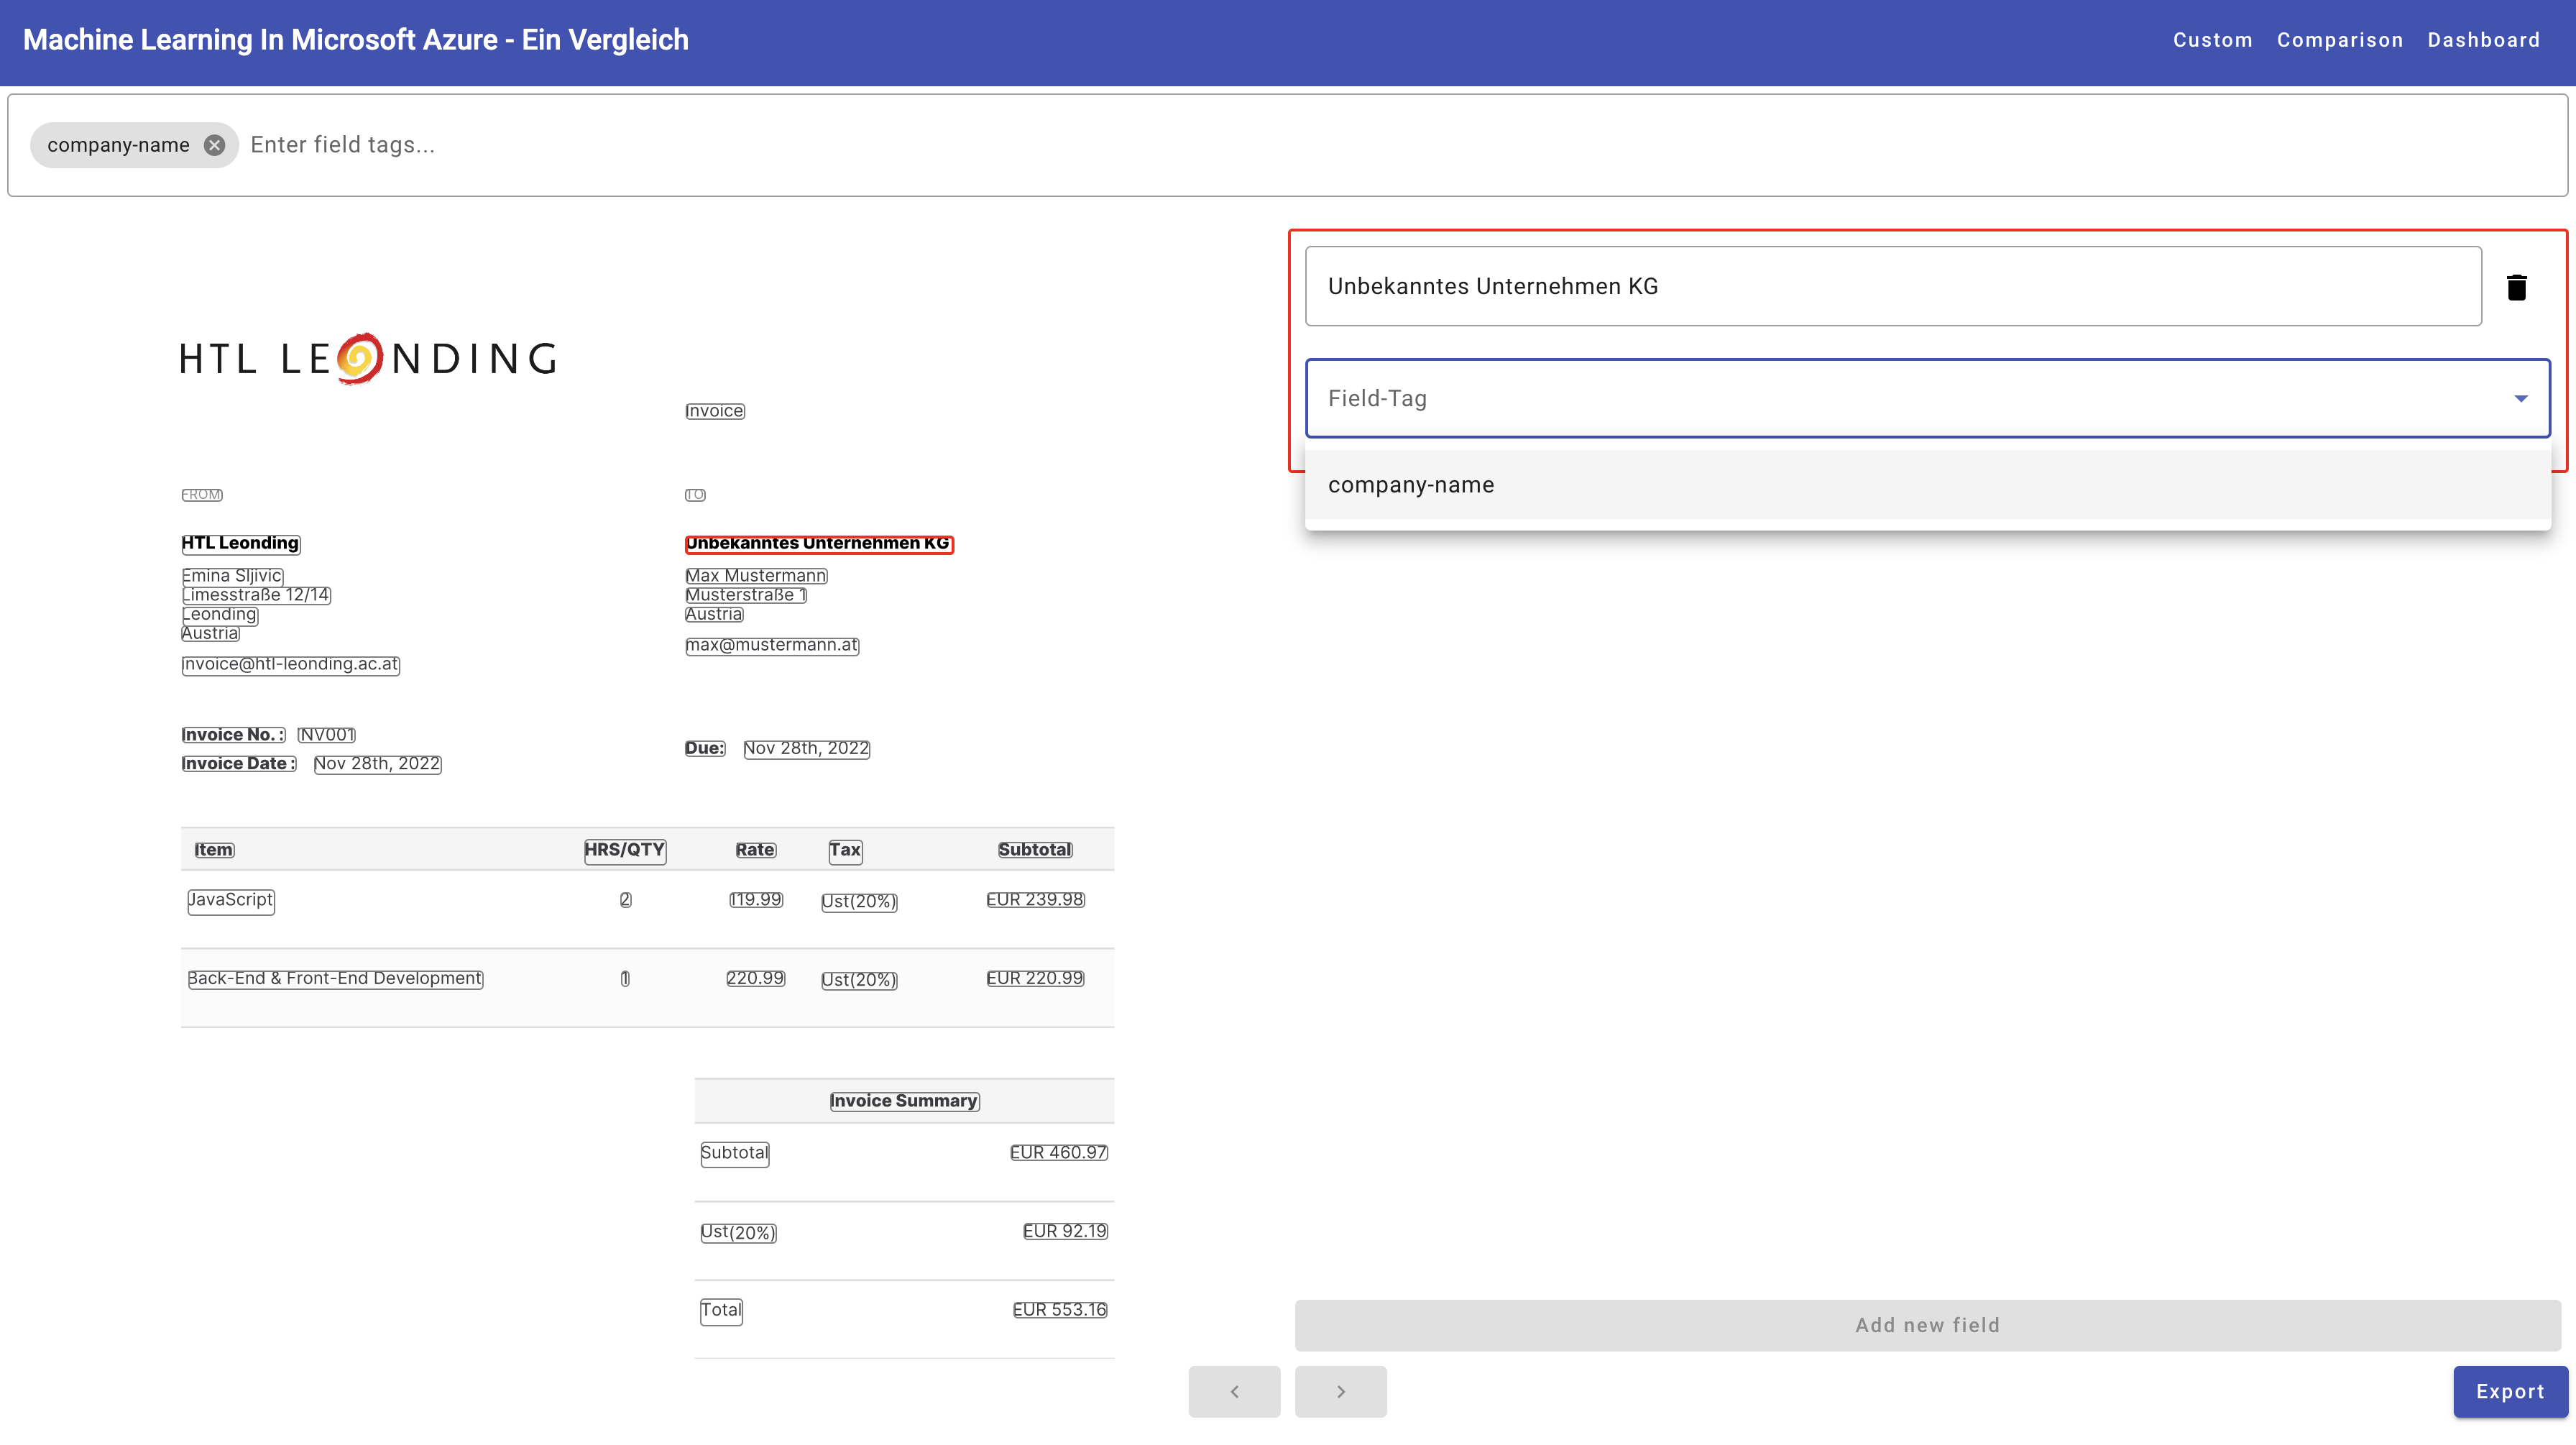
\includegraphics[scale=0.25]{sections/implementation/images/NERAnotationTool.png}
    \caption{NER Annotation Tool mit Beispieldaten}
\end{figure}

Nachdem der User eine oder mehrere Dateien ausgewählt hat, wird im Hintergrund mithilfe von Event-Binding eine Methode ausgelöst, die entweder einen oder mehrere \gls{http}-GET-Requests abschickt. Diese werden als Promise gespeichert, was heißt, dass das Programm auf alle Antworten wartet, bevor es mit dem nächsten Schritt weiter macht. Die Antworten geben die ausgewählten pdf-Dateien als blob-Objekt zurück.

\begin{lstlisting}[language=TypeScript, caption = {HTTP-GET-Requests für die pdf-Dateien}]
    const getImagePromises = this.invoices.map(i => this.http.get(i.url, {responseType: 'blob'}).toPromise());
    const images = await Promise.all(getImagePromises);
\end{lstlisting}

Dieses blob-Objekt wird durch das zusätzlich installierte Paket \lstinline{ng2-pdf-viewer} dargestellt. 

Mit weiteren \gls{http}-Requests werden die Azure Functions aufgerufen, um das pdf-File richtig zu skalieren und um jede Wortgruppe mit einer Box zu umranden. Mithilfe dieser Boxen kann die Rechnung annotiert werden. Jede Annotation besteht aus dem Inhalt der Box und einer Entität, die zuvor im oberen Feld eingegeben wurden. 

Um diese Boxen darzustellen, wird automatisch ein \lstinline{div}-Element über dem pdf-Viewer erstellt und durch den \lstinline{renderer} mit den Boxen gefüllt. Ein \lstinline{renderer} ermöglicht das Eingreifen in den \gls{html}-Struktur über den dahinterliegenden Code.

All diese \gls{http}-Requests werden mit dem über Dependency-Injection initialisierten HttpClient ausgeführt. Dieser Client wird von Angular zur Verfügung gestellt.

Nachdem alle Rechnungen annotiert wurden, können die Annotationen im \lstinline{json}-Format über den 'Export'-Button exportiert werden.

\begin{lstlisting}[caption={Beispiel für eine exportierte json-Datei}]
    {
        "company-name": "Unbekanntes Unternehmen KG",
        "company-address": "Musterstrasse 1",
        "invoice-id": "INVOO01",
        "invoice-date": "Nov 28th, 2022",
        "item-header": "Item",
        "qty-header": "HRS/QTY",
        "rate-header": "Rate",
        "total-header": "Subtotal",
        "total-value": "EUR 553.16"
    }
\end{lstlisting}

\subsubsection{Invoice Reader}

Der Invoice Reader ermöglicht das Extrahieren von Daten aus einer pdf-Datei, daraufhin werden diese Daten im Interface dargestellt.

\begin{figure}[H]
    \centering
    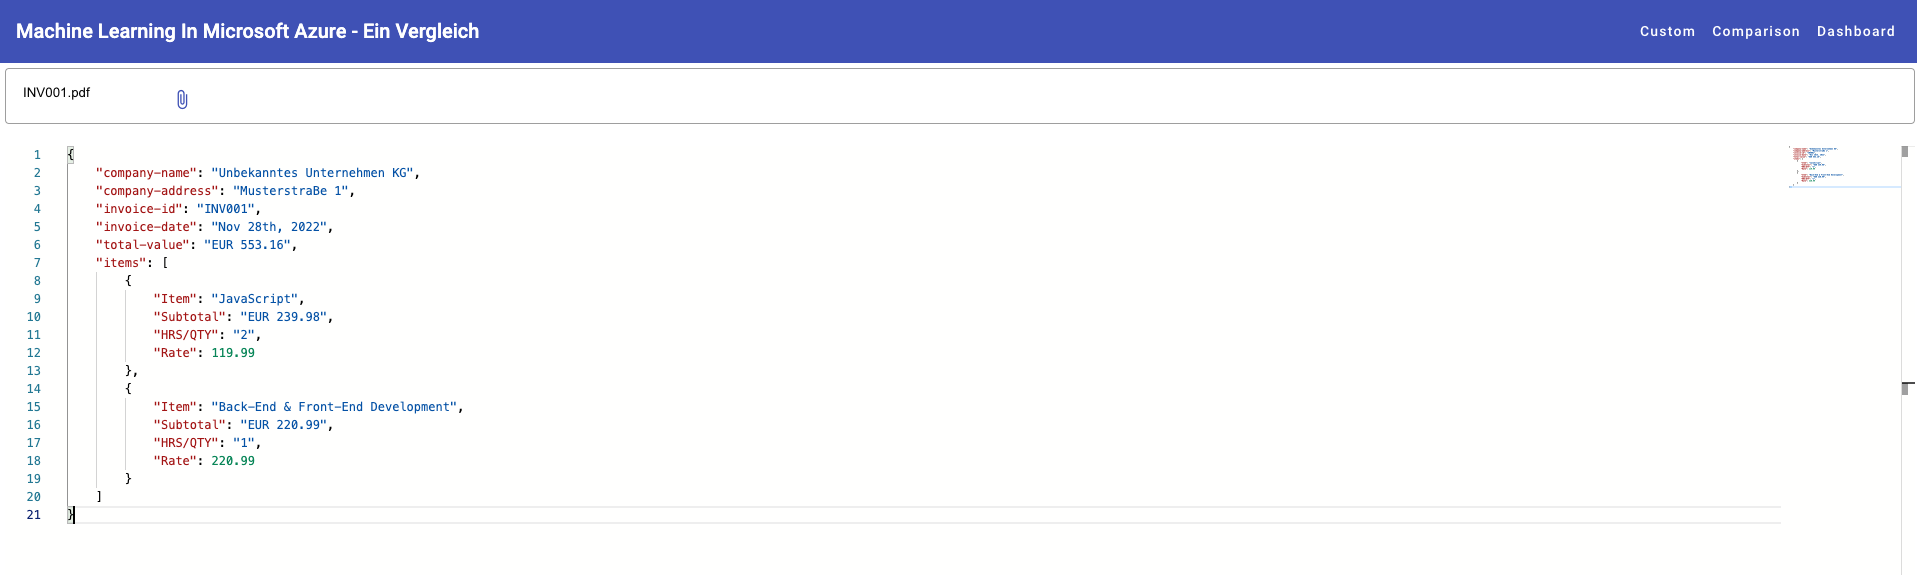
\includegraphics[scale=0.25]{sections/implementation/images/InvoiceReader.png}
    \caption{Invoice Reader mit Beispieldaten}
\end{figure}

Nachdem der User eine pdf-Datei auswählt, wird ein \gls{http}-Request an das Backend abgeschickt und als Antwort wird ein json-Objekt zurückgeliefert, welches die extrahierten Daten enthaltet. Diese Daten werden daraufhin formatiert und in einem monaco-Editor dargestellt.




\begin{spacing}{1}
	\chapter{Zusammenfassung}
\end{spacing}
\setauthor{Emina Sljivic}

\section{Gelerntes}

Dadurch, dass diese Diplomarbeit mein erster Kontakt mit OCR, NER und generell Informationsextraktion war, wurde die meiste Zeit in die Recherche gesteckt. Während der Recherche bin ich auf unterschiedliche Ansätze gestoßen, davon wurden die meisten auch ausgetestet und gleich wieder verworfen, da sie für unseren Anwendungsfall nicht geeignet sind. 

Ein Beispiel dafür war die Tabellenextraktion, bei der drei unterschiedliche Ansätze getestet wurden. Als Erstes wurden Libraries getestet, welche von sich selber die Möglichkeit anbieten, eine ganze Methode zu extrahieren. Jedoch waren diese nicht passend, da unsere Beispieldaten nicht herkömmlich formatiert sind. Das gleiche Problem war der Grund, dass die komplett selbst entwickelte Tabellenextraktion verfallen wurde. 

Außerdem wurde beim Antrainieren des Modells getestet, was die minimale Anzahl der Trainingsdaten ist. Daher wurde das erste Modell mit nur fünf Rechnungen trainiert, wo auch schnell klar wurde, dass dies viel zu wenig sind, da zum Beispiel die Adressen nur zum Teil extrahiert wurden und manche Feld komplett falsch kategorisiert wurden. Daraufhin wurde die Anzahl der Trainingsdaten stufenhaft erhöht und am Ende wurde kam die optimale Anzahl auf rund 15 Rechnungen.

Abgesehen vom technischen Teil wurde mir auch organisatorisch viel für die Zukunft mitgegeben. Da ich im Vorfeld nicht damit gerechnet habe, dass man mehrere unterschiedliche Ansätze austesten muss, bis man den richtigen findet, wurde viel mehr Zeit in die Entwicklung gesteckt, als am Anfang geplant.

\section{Danksagung}

An dieser Stelle möchte ich mich bei all denjenigen bedanken, die mich während der Anfertigung dieser Masterarbeit unterstützt und motiviert haben.

Ich bedanke mich bei jedem Mitarbeiter von smartpoint, die mich in jeglicher Art unterstützt haben. Zusätzlich bedanke ich mich bei smartpoint dafür, dass sie für die Diplomarbeit eine Testumgebung zur Verfügung gestellt haben und dass sie auch nach der Praktikumszeit für Fragen ein offenes Ohr hatten. 

Außerdem möchte ich mich bei Nico Bojer für das mehrmalige Korrekturlesen meiner Diplomarbeit danken. 

Weiters gilt mein Dank meinem Diplomarbeitsbetreuer, Karpowicz Michał, welcher mich auch in stressigen Situationen unterstützt hat.

\newpage
\pagenumbering{Roman}
\setcounter{page}{\value{RPages}}
\newacronym{swt}{SWT}{Stroke Width Transformer}
\newacronym{mser}{MSER}{Maximally Stable Extremal Regions}
\newacronym{icdar}{ICDAR}{International Conference of Document Analysis and Recognition}
\newacronym{ml}{ML}{Machine Learning}

% Usage:
% \gls{label} lowercase in text
% \Gls{label} Uppercase in text
% \newacronym{label}{abbrev}{full}
% \newglossaryentry{label}{settings}



%\setlength{\glsdescwidth}{0.8\linewidth}
\glsnogroupskiptrue
\printglossary[title=Glossar,toctitle=Glossar] %,style=long]
\spacing{1}{
	%\bibliographystyle{IEEEtran}
	\bibliographystyle{ieeetrande}
	\bibliography{bib}
}
\listoffigures
\listoftables
\lstlistoflistings
\end{document}
